% !TEX TS-program = xelatex

\chapter{Geometry and topology primer}
\label{chapt:3}

It is implausible to set up a computer language and computational environment to define and deliver the geometric shape of construction elements and spaces without a pretty good understanding of geometric and topological concepts. Hence, this chapter introduces some basic notions about geometric spaces, operators, and properties, like linearity, that provide the computational foundation of shape definition and model construction.
The essential elements of geometric spaces and cellular models, like affine transformations and simplicial, cubical, polyhedral, and chain complexes, constitute the substrate of discourse for |Plasm| building hierarchical assemblies of AEC products of any scale and complexity.

%1234567890234567890234567890234567890234567890234567890234567890234567890
\section{Geometric Spaces}\label{chapt:3-1}


In mathematics and science, a space is a set of objects with some added structure.
In this section we discuss the geometrical spaces used to represent inside a computer memory the actual objects of natural, artificial or virtual environments, or better their geometric models, in order to study, visualize and/or simulate some associated physical behavior. 
In particular, we deal in this section with linear, affine, and convex spaces as sets of vectors and/or points with selected properties.

\subsection{Vector space}
\label{subsec:2:style}

The concept of vector space is undoubtedly the most helpful instrument of mind invented by mathematicians for scientists, engineers, and architects, to represent and study formally or graphically both the primary and complex arrangements and behaviors of our natural and artificial environment.

\begin{definition}[Vector space] (or \emph{linear space}) $\mathcal{V}$ over a field $\mathcal{F}$ is a set, closed w.r.t. two composition rules (the output of composition belongs to the set of inputs).
\end{definition}

%$+ : \mathcal{V} \times \mathcal{V} \to \mathcal{V}$ \hfill (addition: internal composition)
%
%$\cdot : \mathcal{F} \times \mathcal{V} \to \mathcal{V}$ \hfill (product by a scalar: external composition)
%
%such that, for each $\v{u}, \v{v}, \v{w} \in \mathcal{V}$ and for each scalar $\alpha, \beta \in \mathcal{F}$, the rules $+, \cdot$ satisfy the following
%axioms:
%\begin{quote}
%\begin{enumerate}
%\item  $\v{v} + \v{w} = \v{w} + \v{v}$; \hfill (commutativity of addition)
%\item  $\v{u} + (\v{v} + \v{w})=(\v{u} + \v{v}) + \v{w}$;  \hfill (associativity of addition)
%\item  there is a $\v{0} \in \mathcal{V}$ such that $\v{v} + \v{0} = \v{v}$; \hfill (neutral element of addition)
%\item  there is a $-\v{v} \in \mathcal{V}$ such that $\v{v} + (-\v{v}) = \v{0}$; \hfill (inverse of addition)
%\item $\alpha \cdot (\v{v} + \v{w}) = \alpha \cdot \v{v} + \alpha \cdot \v{w}$; \hfill (distrib. of addition w.r.t. product)
%\item $(\alpha + \beta) \cdot \v{v} = \alpha \cdot \v{v} + \beta \cdot \v{v}$; \hfill (distrib. of product w.r.t. addition)
%\item $\alpha \cdot (\beta \cdot \v{v})=(\alpha \beta) \cdot \v{v}$; \hfill (associativity of product)
%\item $1 \cdot \v{v} = \v{v}$. \hfill (neutral element of product)
%\end{enumerate}
%\end{quote}
%
%The dot operator to multiply a vector by a scalar will be dropped in the remainder of
%this book, so that the operation will be denoted by the juxtaposition of the arguments.
%Hence we write $\alpha(\beta\, \v{v})$ instead of $\alpha \cdot (\beta \cdot \v{v})$.\\

The elements $\v{v}\in \mathcal{V}$ are called \emph{vectors}, and are often represented by an oriented arrow with given direction, orientation, and length. The elements $\alpha\in\mathcal{F}$ are called \emph{scalars}. The sum of two non-zero vectors $\v{u},\v{v}\in\mathcal{V}$ is a third vector $\v{w} = \v{u}+\v{v}\in\mathcal{V}$ with direction and length different from both $\v{u}$ and $\v{v}$.  We may write $\v{v}+\v{v} = 2\v{v}$, and see here both the operations of a vector space: (a) addition of vectors, and (b) multiplication times a scalar. 

The product of a vector by a scalar $\alpha\, \v{v} = \v{v}\, \alpha \in \mathcal{V}$ is a vector collinear with $\v{v}$ and with different length if $\alpha \not= 1$. This explain the name “scalar” since a number “scales” (change the length of) the vector it multiplies. 

The length of $\v{u} = \alpha\,\v{v}$  grows or shrinks w.r.t. $\v{v}$ according to a positive $0 < \alpha < 1$. If $\alpha < 0$, then $\v{u}$ has orientation opposite to $\v{v}$.

%\begin{lstlisting}[language=JuliaLocal, style=julia]
%using Distributions
%
%function thompson_sampling(𝛂, 𝛃, apply; T=100)
%    for t in 1:T
%        𝛉 = rand.(Beta.(𝛂, 𝛃))
%        x = argmax(𝛉)
%        r = apply(x)
%        𝛂[x], 𝛃[x] = (𝛂[x] + r, 𝛃[x] + 1 - r)
%    end
%    return Beta.(𝛂, 𝛃)
%end
%\end{lstlisting}


\subsubsection*{Linear independence}

A \emph{linear combination} of vectors is a new vector that is defined as a sum of scalar multiples of other vectors.
Let $\v{v}_1, \v{v}_2,..., \v{v}_n \in \mathcal{V}$ and $\alpha_1, \alpha_2,...,\alpha_n \in \mathcal{F}$, with $\mathcal{V}$ a vector
space on the field $\mathcal{F}$ of scalar numbers. The vector 
\[
\v{w} = \alpha_1 \v{v}_1 + \alpha_2 \v{v}_2 + \cdots + \alpha_n \v{v}_n = \sum^n_{i=1}
	\alpha_i \v{v}_i \in \mathcal{V}
\]
is called a linear combination of vectors $\v{v}_1, \v{v}_2,..., \v{v}_n$.

\begin{itemize}
\item Two or more vectors are said \emph{linearly independent} if none of them can be written as a linear combination of the others;
\item if at least one of them can be written as a linear combination of the others, then they are said \emph{linearly dependent}.
\end{itemize}

Given a set of vectors, you can determine if they are linearly independent by writing the vectors as the columns of a matrix $\T{A}$, and solving $\T{A}\,\v{x} = \v{0}$. 

If there are non-zero solutions, then the vectors are linearly dependent. If the only solution is $\v{x} = \v{0}$, then they are linearly independent.

The typical vector spaces in this book will be (a) the numeric field $\mathbb{R}$ for scalars and $\mathbb{R}^n$ for vector coordinates, with (b) $\dim = d$, for $0\leq d\leq 3$.

\subsubsection*{Examples}


\begin{coding}[Matrices $m\times n$ are vector spaces].
Generate a random $100\times 100$ matrix |A = rand(100,100)|. The default of |rand()| function are values of type |Float64| in |[0.0,1.0]|, so we ask the compiler to compute the matrix multiplication by the scalar $\pi$, denoted by the Greek symbol. The generated value is shown commented and simplyfied for printing in small space: 

\begin{lstlisting}[language=JuliaLocal, style=julia]
A = rand(100,100) * π 	#=
100x100 Matrix{Float64}:
 0.901069  …  0.172854
 0.357548     0.8537
 ⋮         ⋱  
 0.519136     0.857736 		=#
\end{lstlisting}
\end{coding}

\begin{coding}[Random vector generation.]
Then, we generate a 100-vector of random integers within the interval 
|[0,100]|, by using the Julia |0:100| iterator:

\begin{lstlisting}[language=JuliaLocal, style=julia]
b = rand(0:100, 100) 	#=
100-element Vector{Int64}:
 61
 85
  ⋮
 51			=#
\end{lstlisting}
\end{coding}

\begin{coding}[Multiplication matrix-vector.] This operation is implemented natively and very efficiently for big matrices in Julia, as well the product and the sum of dense matrices (the detail of printing  depends on available space on output screen):
\begin{lstlisting}[language=JuliaLocal, style=julia]
A * b	 	#=
100-element Vector{Any}:
 2786.383421064984
 2554.1378635659034
    ⋮
 2735.1205994270754	=#
\end{lstlisting}
\end{coding}

\begin{coding}[Addition matrix-vector.] 
Conversely, the sum of a matrix with a vector is not a linear operation, so we need to broadcast (. operator) the vector |b| on all columns of |A|:

\begin{lstlisting}[language=JuliaLocal, style=julia]
A .+ b 	 	#=
100x100 Matrix{Float64}:
 61.9011  …  61.1729
 85.3575     85.8537
  ⋮       ⋱  
 51.5191     51.8577	=#
\end{lstlisting}
\end{coding}

Summing up: while the |Matrix| by |Vector| multiplication is a native operation on the linear space of |Number|s, The addition of |Matrix| and  |Vector| is not, and the broadcast operator must be used. Same for the sum of a matrix and a single scalar value. The reader should try.


\subsubsection*{Subspace}

Let $\cal V}$ be a vector space on the field ${\cal F}$. 
We say that ${\cal U}\subset{\cal V}$ is a \emph{subspace} of ${\cal V}$ if $\cal U$ is a vector space with respect to the same operations. In particular, ${\cal U}\subset{\cal V}$ is a \emph{subspace} of ${\cal V}$ if and only if:

\begin{enumerate}
\item  ${\cal U}\neq\emptyset$;

\item for each $\alpha\in {\cal F}$ and $\v{u}_1,\v{u}_2\in{\cal U}$, $\alpha \,\v{u}_1+\v{u}_2 \in{\cal U}$
\end{enumerate}

The \emph{codimension} of a subspace ${\cal U}\subset{\cal V}$ is 
defined as $\dim{\cal V} - \dim{\cal U}$.

It may be useful to note that the intersection of subspaces is a subspace.
In particular, if ${\cal U}_1,{\cal U}_2$ are subspaces of ${\cal V}$, then ${\cal U}_1\cap{\cal U}_2$ is a subspace of ${\cal V}$.


\subsubsection*{Generators, Bases, and Coordinates}

\subparagraph*{Span and generators}
The smallest subset of vectors that can be generated by linear combinations of a subset ${S}\subset\mathcal{V}$ of linearly independent vectors is called  $span\,{S}$.

The set ${S}$ is therefore called a set of \emph{generators}.

The $span\,{S}$ is closed with respect to addition and multiplication, and hence is a \emph{subspace} including the zero vector, which is contained in every subspace. 


\subparagraph*{Bases and coordinates}

The \emph{basis} and \emph{dimension} of the linear space $\mathcal{V}$ are a minimum set of generators for $\mathcal{V}$, and its number $d = \dim\mathcal{V}$ of elements, respectively. 

Every basis of a linear space $\mathcal{V}$ has the same number $d$ of elements. 

When a basis for $\mathcal{V}$ has been fixed, i.e. an ordered minimal subset of generators ${B} \subset \mathcal{V}$  has been chosen, every vector $\v{v}\in \mathcal{V}$ can be expressed \emph{uniquely} as the linear combination of elements of ${B}$ with scalars. The ordered tuple of such scalars is called the \emph{coordinate} tuple, or the coordinates, of vector $\v{v}\in\mathcal{V}$, and denoted as $[\v{v}]$.  

\begin{remark}
It is to mention that to represent vectors by coordinates requires that a minimum set of space generators and their ordering have been already chosen. We will say that the space has been p\emph{arameterized}, since every vector is \emph{uniquely} identified by the linear combination of the basis elements with a unique tuple of scalars. 
\end{remark}

\begin{remark}
The basis is often denoted by the ordered sequence $(\v{e}_1,\ldots,\v{e}_d)$ of vector elements, or by the matrix $[\v{e}_1 \cdots \v{e}_d]$ of their coordinates by columns, where $\v{e}_i = [0, 0, 1, \ldots, 0]^t$ is a (column) tuple of zeroes, with only one element $1$ in position $i$. The \emph{standard basis} of a coordinate vector space is the set of vectors whose components are all zero, except one that equals 1.
\end{remark}




\subsubsection*{Examples of vector spaces} 

The usual geometric example of vector space has the oriented arrows\footnote{Formally: the equivalence classes of equipollent oriented arrows. In Euclidean geometry, equipollence is a binary relation between directed line segments. } as elements, summed with the parallelogram rule, and scaling related to elongation or shortening.
Other examples are the linear spaces of matrices $\mathcal{M}^n_m(\mathbb{R})$ with real elements, $m$ rows and $n$ columns, and $\mathcal{M}_m(\mathbb{R})$ and $\mathcal{M}^n(\mathbb{R})$ of column and row vectors, respectively.

Linear space is also the space $\P_n(\mathbb{R})$ of real polynomial functions $p: \mathbb{R}\to\mathbb{R}$ such that $x\mapsto p^n(x)$ of degree $\leq n$. In particular, $p^n(x) = a_0 + a_1\, x + a_2\, x^2+ \cdots + a_{n-1}\, x^{n-1} + a_{n}\, x^n$ is exactly a linear combination of a tuple of $n+1$ scalars $a_k$, $0\leq k\leq n$, with the \emph{power basis} of polynomials $x^k$, $0\leq k\leq n$. 


\subsubsection*{The Bernstein bases of polynomial space $\P_n(\R)$}

In geometric modeling and computer graphics, the Bernstein-Bézier basis of polynomials is fundamental. The $n+1$ Bernstein polynomials of degree $n$, defined as
\[
B^n_k(x) = {n \choose k}\,x^k\,(1-x)^{n-k}, \qquad 0\leq k \leq n
\]
form a basis for the vector space $\P_{n}(\R)$ of polynomials of degree at most $n$ with real coefficients. Therefore, to implement the basis and to draw a graph of each basis function we have to consider: the degree |n| we are interested to; the ordinal number |k| of each function ($1\leq k\leq n$); and finally the independent variable $x$ such that $x \mapsto p^n(x)$. 

\begin{coding}[Pure functional style in Julia]
The julia function |B| \\ given here returns the whole range of Bézier-Bernstein polynomial bases of any degree, and is very useful in curve geometric modeling.
\lstinputlisting[language=JuliaLocal,style=julia,mathescape=false]{/Users/paoluzzi/Documents/dev/PLASM/SPRINGER/BOOK/chapter-02/src/001.jl}
This pure programming style is available in Julia and will be adopted when useful to get curried applications of functions. 
\end{coding}


Let us make some checks: |B(1)(0)(0.5) == B(1)(1)(0.5) == 0.5 #=> true|,  for the degree-1 basis  made by polynomials |B(1)(0)| and |B(1)(1)|.  The vhole basis of degree $n$ is generated by the higher-level function |Bernstein(n)| that we test in the quadratic case, where it returns a 3−element array of |Vector{Function}|:
\begin{coding}[Generating Bernstein polynomial bases]
The function |Bernstein(n)| is defined by mapping the partial function |B(n)| over the integer array |[0, 1, ..., n ]|. 
\lstinputlisting[language=JuliaLocal,style=julia,mathescape=false]{/Users/paoluzzi/Documents/dev/PLASM/SPRINGER/BOOK/chapter-02/code/002.jl}
\end{coding}


Now, we go to generate a discrete sequence of functions for the “vector” function |Bernstein(2)|, in order to test the implementation. 
Above we see also the second function of Bernstein basis of degree |n=2|, and finally its value |0.18| computed for |x = 0.1|. 

\begin{coding}[Sampling of third quadratic polynomial] The function |Bernstein(2)[3]| denotes the third  function of the vector array |Bernstein(2)| of type |::Vector{Function}|, and we compute the three function values for |x=0.5|, that you can check in Figure~\ref{}.

\lstinputlisting[language=JuliaLocal,style=julia,mathescape=false]{/Users/paoluzzi/Documents/dev/PLASM/SPRINGER/BOOK/chapter-02/code/003.jl}
\end{coding}



\begin{coding}[Sampling of third basis polynomial of degree 4]. We may look at the sequence of pairs $x, Bernstein(2)[3](x)$. A sampling of $x$ values is created by |collect(0:0.1:1)|:
\lstinputlisting[language=JuliaLocal,style=julia,mathescape=false]{/Users/paoluzzi/Documents/dev/PLASM/SPRINGER/BOOK/chapter-02/code/004.jl}
\end{coding}



The Bernstein basis enjoy interesting properties. They are $\geq 0$ for every value of the independent variable $x\in [0,1]$. Even more, for every $x$ the elements of each basis sum to 1. Such bases are said \emph{partition of unity}. 

\begin{figure}[htbp] %  figure placement: here, top, bottom, or page
   \sidecaption[t]
   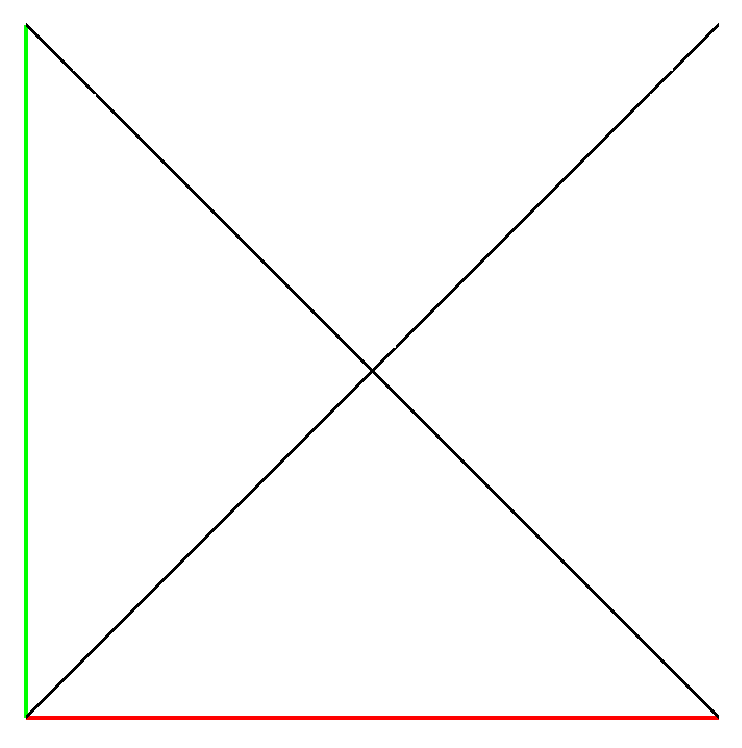
\includegraphics[height=0.25\linewidth,width=0.25\linewidth]{chapter-03/figs/bernstein1}%
   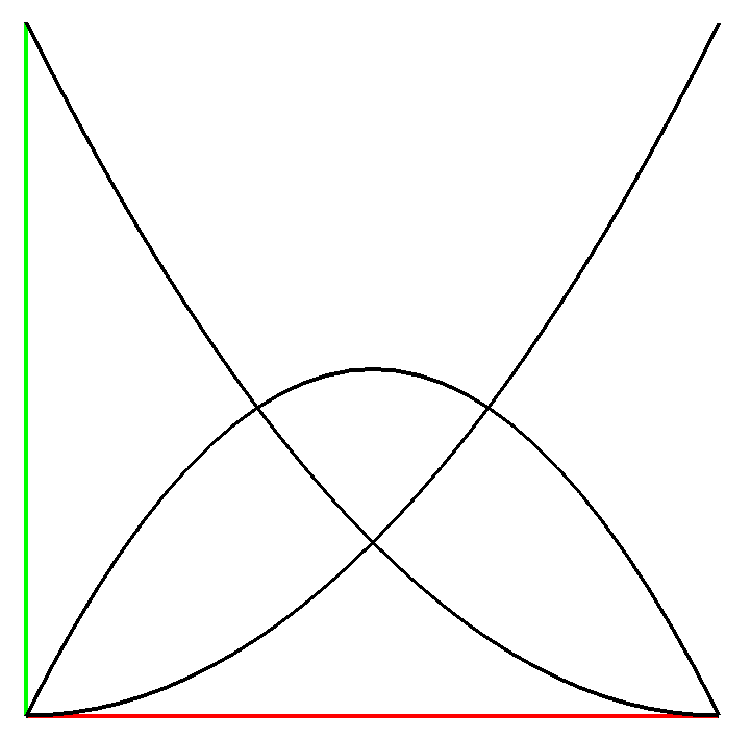
\includegraphics[height=0.25\linewidth,width=0.25\linewidth]{chapter-03/figs/bernstein3}%
   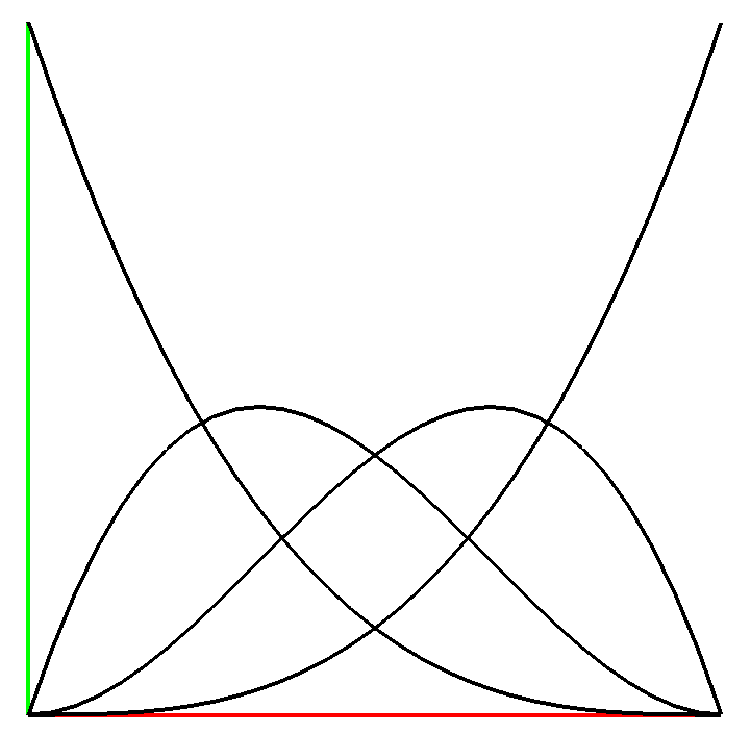
\includegraphics[height=0.25\linewidth,width=0.25\linewidth]{chapter-03/figs/bernstein2}%
   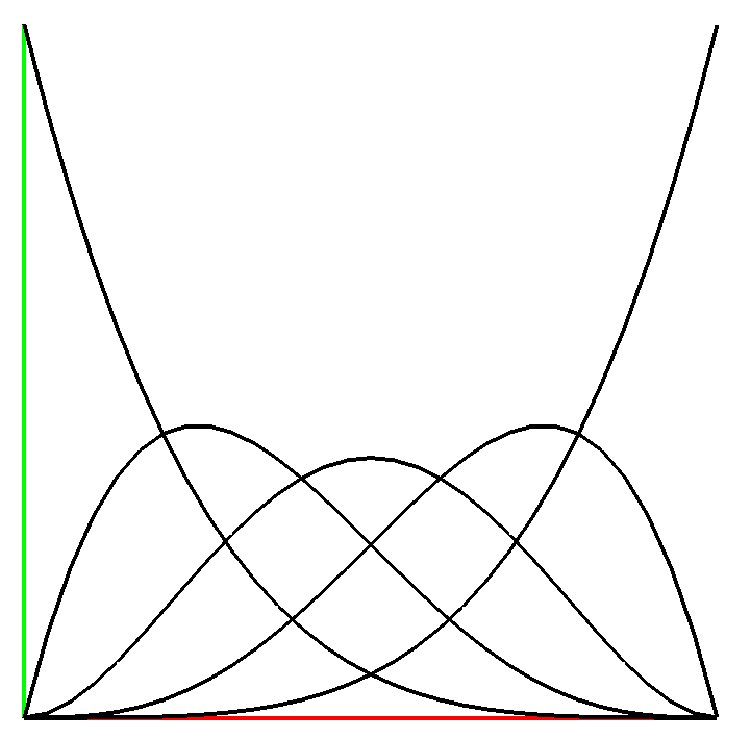
\includegraphics[height=0.25\linewidth,width=0.25\linewidth]{chapter-03/figs/bernstein4}%
   \caption{The four images give the graph, in $[0,1]\times[0,1]\subset\mathbb{E}^2,$ of Bernstein’s basis of linear, quadratic, cubic, and quartic polynomials in linear spaces $ 
   \P_n(\R)$, with $1\leq n\leq 4$, and $\dim(\P_n(\R)) = n+1 = {}$2, 3, 4, and 5, respectively.}
   \label{fig:bernstein}
\end{figure}  


\begin{coding}[Example of \texttt{FL \& Plasm} Combinators]
We remark on the incredible expressive power of |FL| programming inherited in |Plasm.jl|.

It is greatly useful to analyze goals and types of subexpressions, recuperating backward the development process to  write the result expression.
First, we define the 1D model |dom1D| of the function domain $[0,1]$ with 36 intervals, which is a geometric value of |Hpc| type:

\begin{lstlisting}[language=JuliaLocal, style=julia]
dom1D = INTERVALS(1.0)(36)  	#=
Hpc(MatrixNd([[1.0, 0.0], [0.0, 1.0]]), BuildMkPol[BuildMkPol(points=[[0.0], [0.027777777777777776], ... =#
\end{lstlisting}

Then, consider the $\E\to\E^2$ vector function |CONS(...)∘S1| of one variable, that is applied to the vertices of |dom1D::Hpc| by the |MAP| operator. 

The selector function |S1| is used to extract the first (and unique) coordinate value from the internal data structure |point| array. The |CONS| operator, acting on argument of |Vector{Function}| type, transforms a  function array into a vectorial function of coordinate functions |x(u)|, |y(u)|, etc. 

Hence, we have |F = CONS(::Vector{Function})∘Sd|${} : \E^d\to\E^n$, where |d| is the number of coordinates of domain vertices (one in this case), and |n| is the dimension of the embedding space, i.e., the number of coordinate functions inside the array argument, i.e.~|CONS([,])|, two in this case:

\begin{lstlisting}[language=JuliaLocal, style=julia]
F(k) = CONS([ID, Bernstein(4)[k]])∘S1		#=
#122 (generic function with 1 method)	=#
\end{lstlisting}

Finally, we note that expressions like |MAP(F)(dom1D)| are used to apply the |F| vector function to an object of |Hpc| type, normally to bend it.
Remember that we  generated an array of |Hpc| curves, for |k=1:n+1| --- in our case with |n=4|. For this purpose, we need to finally apply the |STRUCT| operator, to transform the array of curves into a single |Hpc| value.
\begin{lstlisting}[language=JuliaLocal, style=julia]
STRUCT( MAP(F(k))(dom1D) for k=1:n+1 )
\end{lstlisting}

\end{coding}


\subsubsection*{Change of basis} 

It is often necessary, given a basis in a linear space, to compute a novel parameterization of the space with respect to a different, possibly more simple or useful basis. In other words, may be necessary to compute new coordinates for the vectors of the space, with respect to a new basis. This operation is called \emph{change of basis}. 

For concreteness, let we have vector data in a 3D linear space, where we need to compute their representation in a different basis. Let us denote the new basis as $(\v{u}_i)$, and the standard one as $(\v{e}_i)$, with $i\in \{1,2,3\}$. We may write the change of coordinates as a matrix map $\T{T}: \mathcal{V}\to\mathcal{V}$, such that $[u_{ij}] \mapsto [e_{ij}]$, so transforming the old coordinates of the new basis into the standard basis. 

Therefore we set $\T{T}\, [u_{ij}] = [e_{ij}]$ and, since it is $[e_{ij}]={I}_{3}$, i.e., the $3\times 3$ identity matrix, the solution is $\T{T}=[u_{ij}]^{-1}$. Of course, this matrix exists provided that $\det\, [u_{ij}] \not= 0$. In other words, the vectors of the new basis must be linearly independent.


\subsection{Affine space}
\label{subsec:2:style}

In geometric modeling and computer graphics it is useful to distinguish between a space of vectors and a space of points (supported by vectors). A space of points, that provides for an operation of \emph{displacement}, is called an \emph{affine space}, and is represented here by the $\mathcal{A}$ symbol. In particular, we call \emph{affine action}  the function:
\[
\mathcal{A} \times \mathcal{V} \to \mathcal{A},
\]
so that  the \emph{displacement} from a point $\p{a} \in \mathcal{A}$ to a point $\p{b} \in \mathcal{A}$ is given. An affine space $\mathcal{A}$ is endowed with an operation of \emph{difference} of points $\mathcal{A} \times \mathcal{A} \to \mathcal{V}$ where
\[
\p{a} + \v{v} = \p{b}, \quad\mbox{and hence}\quad \p{b}-\p{a} = \p{v} \in \mathcal{V} 
\]

\subsubsection*{Remarks}
\label{sec:ccccccc}

We note that a \textbf{vector space} provides   for an internal operation of (a) \emph{sum} of two vectors and the external (b) \emph{product} of a vector by a scalar, both returning a vector. Conversely, in an \textbf{affine space} we have an external operation of (i) \emph{difference} of points, returning a vector, and  a (ii) sum of a point and a vector, called \emph{displacement}, returning a point.

Even more, in a vector space $\mathcal{V}$ there is a distinguished element $0$, the \emph{zero vector}, which is contained in all subspaces. On the contrary, in an affine space $\mathcal{A}$ \emph{all points are equivalent}, with no distinguished elements. 

We usually say that a space of points has been parameterized when a \emph{Cartesian system} (origin and basis) has been chosen.
In order to use coordinates to make it easier to work with points we have to choose :

\begin{enumerate}
\item 
a point, called \emph{origin}, to associate with the zero vector, and 
\item 
an orthonormal \emph{basis} of vectors. 
\end{enumerate}

The above steps consent to associate each point with the tuple of coordinates of its \emph{displacement vector} from the origin. 

In a vector space all the subspaces have at least a common element, the zero vector. Contrariwise, two affine subspaces may not have common elements. In such a case they are said \emph{parallel}. 

The dimension $n$ of an affine space $\mathcal{A}$ is that of its supporting vector space $\mathcal{V}$.
A common word for \emph{affine subspaces} of $d$ dimension is $d$-hyperplane, or $d$-hyperspace when $d>3$. Lines and planes are affine subspaces of dimension $1$ and $2$, respectively. 


\subsubsection*{Affine independence and local parameterization}
\label{sec:ccccccc}

In an affine space $\mathcal{A}$ of sufficiently high dimension $n$ we say that two points are \emph{affinely independent} when \emph{non coincident}, three points when \emph{non aligned}, four points when \emph{non coplanar}, and so on. 

In general, $d+1$ points  ($d \leq n$) are affinely independent when the $d$ vectors defined by the differences $\p{p}_k - \p{p}_0$ of points from one of them are linearly independent. 

The affine independence of a subset of $d+1$ points is often used to establish \emph{local coordinate systems} on lines, planes and higher dimensional subsets of points. Let us choose two non coincident points $\p{a},\p{b}$ on a 3D line. Any other point $\p{p}$ of the line remains parameterized by the $\alpha$ scalar in the expression 
\[
\p{p} = \p{a} + \alpha(\p{b}-\p{a}). 
\]
Note that $\p{b}-\p{a}$ is a vector, $\alpha(\p{b}-\p{a})$ is a vector, $\p{a} + \alpha(\p{b}-\p{a})$ is a point plus a vector, which is a point. The typing of our expression looks correct!

Analogously, let us choose three non colinear points $\p{a},\p{b},\p{c}$ in 3D space. They are certainly non coincident, and of course fix a plane, i.e., an unique affine subspace of dimension 2 embedded in space. A parameterization of this plane is given by the pairs $(\alpha,\beta)$ of scalars in the expression
\[
\p{q} = \alpha(\p{b}-\p{a}) + \beta(\p{c}-\p{a}),
\] 
as the reader may immediately check. Similar local coordinates will hold in every affine $d$-subspace in $n$-dimensional space.

The typical affine space of points used in this book is the Euclidean space $\mathbb{E}^d$, $1 \leq d \leq 3$, usually furnished of a Cartesian system, with coordinates in |Float64|.



\subsection{Convex space}
\label{subsec:2:style}

Let us consider the Euclidean space $\mathbb{E}^d$, $d\in\{2,3\}$ affine over the reals, that is the fundamental space of geometry, intended to represent physical space. 

Affine subspaces become \emph{convex sets} when a numeric constraint is imposed on the possible parameter values of an affine combination of points. Two points $\p{a},\p{b}\in\mathcal{A}$ become the extreme elements of a \emph{line segment} $\p{p} = \alpha\,\p{a} + (1-\alpha)\,\p{b}$ as set of points, by adding the further constraint $\alpha + \beta=1$ to the parameter values $\alpha,\beta \geq 0$, so posing $\beta=1-\alpha$. Analogously, setting $\alpha + \beta + \gamma = 1$ and $\alpha, \beta, \gamma \geq 0$ constraints the set of points combination of three non aligned points $(\p{a}, \p{b}, \p{c})$. 


\subsubsection*{Positive, Affine and Convex Combination of Points}
\label{par:AffineConvexCombination}

Let $\p{p}_1, \p{p}_2, \ldots, \p{p}_n$ be affinely independent points in $\mathbb{E}^d$, and $\alpha_1, \alpha_2, \ldots, \alpha_n$ be scalar in $\mathbb{R}$. Their combination $\alpha_1 \p{p}_1 + \alpha_2 \p{p}_2 + \cdots + \alpha_n \p{p}_n$ is said \emph{positive}, \emph{affine}, and \emph{convex}, respectively, when
\begin{enumerate}
\item $\alpha_1, \alpha_2, \ldots, \alpha_n \geq 0$ \hfill (positive combination)
\item $\alpha_1 + \alpha_2 + \cdots + \alpha_n = 1$ \hfill (affine combination)
\item $\alpha_1 + \alpha_2 + \cdots + \alpha_n = 1\quad\mbox{and}\quad \alpha_1, \alpha_2, \ldots, \alpha_n \geq 0$ \hfill (convex combination)
\end{enumerate}

It may be interesting to verify that the affine combination of points is a point.
Let us eliminate the $\alpha_1$ scalar using the unitary sum of scalars constraint:
\begin{eqnarray}
\p{p} = (1 - \alpha_2 - \cdots - \alpha_n) \p{p}_1 + \alpha_2 \p{p}_2 + \cdots + \alpha_n \p{p}_n\\
= \p{p}_1 + \alpha_2 (\p{p}_2-\p{p}_1) + \cdots + \alpha_n (\p{p}_n-\p{p}_1)
\end{eqnarray}
which, of course, is a point in $\mathbb{E}^d$.

A convex combination is positive and affine.

The set of all convex combinations of points $C \subset \mathbb{E}^n$ is the \emph{convex hull} of $C$.  The convex hull is the smallest compact set containing the points in $C$.
It is the intersection of all compact sets of $\mathbb{E}^d$ which contain $\mbox{hull}\, C$. 

\emph{Convex coordinates} of a point $\p{c} \in \mbox{hull}\, C$ are the scalars whose convex combination with $C$ elements produces $\p{c}$. If $C\subset \mathcc{E}^n$ has $n+1$ affinely independent elements, i.e., it is a simplex (see Section \ref{sec:simplex}) the convex coordinates of each $\p{c} \in \mbox{hull\ } C$ are \emph{unique}.


\subsubsection*{Characterization of affine pyramids}
\label{sec:ccccccc}

Speaking of local parameterization of affine subspaces, we did not fix any constraint on the signs of the scalar parameters (usually in the field $\mathbb{R}$ of reals). If all the scalars are positive, then all the spanned points stay inside the interior of a planar (or solid) angle contained within the lower-dimensional affine subspaces generated. It would be not difficult to see that the whole subspace will be partitioned by an arrangement of subspaces centered on the fixed point of the set of linearly independent vectors. As an example, consider the partitioning of 3D space generated by the $8 = 2^3$ octants defined by $4$ non coplanar points, and in particular those generated when three points are at unit distance by the first, and the three difference vectors are pairwise orthogonal.

\subsubsection*{Positive, Affine and Convex coordinates}

%12345678901234567890123456789012345678901234567890123456789012345678901234567890

Affine Coordinates for Convex Sets

Barycentric Coordinates for Convex Sets

Test for boundary points: interior and exterior









\section{Cellular models}\label{sect:3-2}


This section discusses computational topology concepts used to compute the 2D/3D space partition induced by a collection of geometric objects of dimension 1D/2D, respectively. Cellular models are are often called \emph{meshes} in engineering and design jargon. A mesh is a representation of a domain by discrete cells. In many areas of geometric/numeric computational engineering, including geo-mapping, computer vision and graphics, finite element analysis, medical imaging, geometric design, and solid modeling, one has to compute incidences, adjacencies and ordering of mesh cells, generally using disparate and incompatible data structures and algorithms. Only sparse vectors and matrices are used in |Plasm| to compute the linear spaces of chains, called chain complex, from dimension zero to three.

\subsection*{Topological definitions}\label{sect:3-2-1}

A \emph{complex} is a graded set $S = \{ S_i \}_{i\in I}$ \emph{i.e.}~a family of sets, indexed here over $I = \{0,1,2,3\}$.
We use two different but intertwined types of {complexes}, and specifically complexes of \emph{cells} and complexes of \emph{chains}. 
Their definitions and some related concepts are given in this section. Greek letters are used for the {cells} of a space partition, and roman letters for {chains} of cells, coded as either (un)signed integers or sparse arrays of (un)signed integers.  


\begin{definition}[$d$-Manifold]
A \emph{manifold} is a topological space that resembles a flat space locally, \emph{i.e.}, near every point. 
Each point of a $d$-dimensional manifold has a neighborhood that is homeomorphic\footnote{Homeomorphic means opologically equivalent.} to $\E^d$, the Euclidean space of dimension $d$. Hence, this geometric object is often referred to as $d$-manifold. 
\end{definition}
\emp{Homeomorphic} neighborhood means “topologically equivalent”, like a rubber patch, that can be stretched without changing its topology.
%\end{paragraph}

\begin{definition}[Cell]
A \emph{$p$-cell} $\sigma$ is a $p$-manifold with boundary ($0\leq p\leq d$) which is 
piecewise-linear, connected, possibly non convex, and not necessarily contractible. This definition refers to cellular complexes used in this paper and is different from other ones because a cell is neither simplicial, nor convex, nor contractible.
\end{definition}
In |Plasm|, cells may contain internal holes; cells of CW-complexes~\cite{hatcher:2002} are, conversely,  contractible to a point.  
We deal with \emph{Piecewise-Linear} (PL) cells of dimensions 0, 1, 2, and 3, respectively. It should be noted that 2- and 3-cells may contain holes, while remaining connected.  In other words, |Plasm| cells are $p$-polyhedra, \emph{i.e.}~segments, polygons and polyhedrons embedded in 2D or 3D space. 
%%\end{definition}

\begin{definition}[Cellular complex]
A \emph{cellular $p$-complex} is a finite set of cells that have at most dimension $p$, together with all their $r$-dimensional boundary faces ($0\leq r\leq p$). A \emph{face} is an element of the PL boundary of a cell, that satisfy the \emph{boundary compatibility} condition. Two $p$-cells $\alpha, \beta$ are said boundary-compatible when their point-set intersection contains the same $r$-faces ($0\leq r\leq p$) for both $\alpha$ and $\beta$. 
\end{definition}
A cellular $p$-complex is said {\emph{homogeneous} }when each $r$-cell ($0\leq r\leq p$) is face of a $p$-cell. 

\begin{definition}[Skeleton]
The $s$-skeleton of a $p$-complex $\Lambda_p$ ($s\leq p$) is the set $\Lambda_s\subseteq\Lambda_p$ of all $r$-cells ($r\leq s$) of $\Lambda_p$. Every skeleton of a regular complex is a regular subcomplex.
The difference $\Lambda_r - \Lambda_{r-1}$ of two skeletons is the set $U_r$ of $r$-cells. 
\end{definition}

\begin{definition}[Support space]
The support space $\Lambda$ of a cellular complex is the point-set union of its cells. 
\end{definition}

\begin{definition}[Characteristic function]
Given a subset $S$ of a larger set $A$, the characteristic function $\chi_A(S)$, also called the \emph{indicator function}, is the function defined to be identically one on $S$, and zero elsewhere. \cite{Wolfram}.
\end{definition}


\subsection{Simplicial complex}\label{sect:3-2-1}


\begin{definition}[Join operation.]
\index{Simplex}
The {\em join} of two compact sets of points $P,Q\subset\E^n$ is the set $PQ$ of convex combinations of points in $P$  and in $Q$.
The join operation is associative and commutative.  
\end{definition}


\begin{definition}[Simplex.]
A {\em $d$-simplex} $\sigma_{d}\subset \E^n$ ($0\leq d\leq n$) may be
defined as the repeated join of $d+1$ affinely independent points,
called {\em vertices}.  
\end{definition}
A $d$-simplex can be seen as a $d$-dimensional
triangle: a $0$-simplex is a \emph{point}, a $1$-simplex is a
\emph{segment}, a $2$-simplex is a \emph{triangle}, a $3$-simplex is a
\emph{tetrahedron}, and so on.


\begin{coding}[Plasm $d$-dimensional simplex]  A $d$-simplex is generated by the |Plasm| package by the |SIMPLEX| multi-dimensional function:
\begin{lstlisting}[language=JuliaLocal, style=julia, mathescape = true] 
julia> using Plasm

julia> SIMPLEX::Function
SIMPLEX (generic function with 1 method)
\end{lstlisting}
\end{coding}


\begin{coding}[Dataset associated to simplices.] The simplex datasets follow, for the first integer parameters. Note that |SIMPLEX(d)| contain $d+1$ coordinate points of dimension $d$, and that |hulls| fields contain $d+1$ indices of points, i.e. a single \emph{convex} cell:
\begin{lstlisting}[language=JuliaLocal, style=julia, mathescape = true]
SIMPLEX(0)			#=
Hpc(MatrixNd(1), Geometry([Float64[]], hulls=[[1]])) =#

SIMPLEX(1)			#=
Hpc(MatrixNd(2), Geometry([[0.0], [1.0]], hulls=[[1, 2]])) =#

SIMPLEX(2)			#=
Hpc(MatrixNd(3), Geometry([[0.0, 0.0], [1.0, 0.0], [0.0, 1.0]], hulls=[[1, 2, 3]])) =#

SIMPLEX(3)			#=
Hpc(MatrixNd(4), Geometry([[0.0, 0.0, 0.0], [1.0, 0.0, 0.0], [0.0, 1.0, 0.0], [0.0, 0.0, 1.0]], hulls=[[1, 2, 3, 4]])) =#

SIMPLEX(4)			#=
Hpc(MatrixNd(5), Geometry([[0.0, 0.0, 0.0, 0.0], [1.0, 0.0, 0.0, 0.0], [0.0, 1.0, 0.0, 0.0], [0.0, 0.0, 1.0, 0.0], [0.0, 0.0, 0.0, 1.0]], hulls=[[1, 2, 3, 4, 5]])) =#
\end{lstlisting}
\end{coding}

For the sake of visual simplicity, we remove the |julia>| prompt for Plasm scripts, and use the multilinear comment to reduce their visual rumor.


\begin{definition}\emph{Skeleton and Faces.}
The set $\{ \p{v}_0, \p{v}_1, \ldots, \p{v}_d \}$ of vertices of
$\sigma_{d}$ is called the {\em 0-skeleton} of $\sigma_{d}$.  The
$s$-simplex generated from {\em any} subset of $s+1$ vertices ($0\leq
s\leq n$) of $\sigma_{d}$ is called an {\em $s$-face} of $\sigma_{d}$.
\end{definition}
\begin{remark}
Let us notice, from the definition, that a simplex may be considered
both as a purely \emph{combinatorial object} and as a \emph{geometric object}, i.e.
as the compact point-set defined by the convex hull of a discrete set
of points.
\end{remark}


\begin{definition}[Simplicial Complex]
A set $\Sigma$ of simplices is called a {\em triangulation}.  
A {\em simplicial complex}, often simply denoted as \emph{complex}, is
a triangulation $\Sigma$ that verifies the following conditions:
\begin{enumerate}
\item
if $\sigma \in \Sigma$, then any face of $\sigma$ belongs to $\Sigma$;

\item
if $\sigma,\tau\in \Sigma$, then either $\sigma\cap
\tau=\emptyset$, or $\sigma\cap\tau$ is a face of both $\sigma$ and
$\tau$.
\end{enumerate}
\end{definition}

A simplicial complex can be considered a \emph{well-formed}
triangulation.  Such kind of triangulations are widely used in
engineering analysis, e.g., in topography or in finite element
methods.

\begin{coding}[binomial numbers and simplex faces]
There are 
\[
\sum_{k=0}^{n} {n \choose k} = 2^n
\] 
$k$-faces in a $n$-simplex. Testing this statement is simple and very elegant with Julia. 
We may verify, e.g., that |simplex(5)| faces are a set of |$2^5$| elements:
\begin{lstlisting}[language=JuliaLocal, style=julia, mathescape = true]
julia> [binomial(5,k) for k=0:5]'
1×6 adjoint(::Vector{Int64}) with eltype Int64:
 1  5  10  10  5  1

julia> [binomial(5,k) for k=0:5] |> sum == 2^5
true
\end{lstlisting}


\end{coding}

\begin{coding}
A simple coding example produces the simplicial complex providing the triangulation of the boundary of a convex hull. 
\begin{lstlisting}[language=JuliaLocal, style=julia, mathescape = true]
julia> p = rand(6,3)				#=
6×3 Matrix{Float64}:
 0.456121  0.340689  0.523394
 0.670731  0.920846  0.810581
 0.511325  0.83709   0.765548
 0.27295   0.344676  0.246891
 0.155611  0.262588  0.372059
 0.997037  0.689132  0.594624		  =#
\end{lstlisting}
The |p| matrix holds 6 random |3D| points. The |q| matrix receives an array of arrays:
\begin{lstlisting}[language=JuliaLocal, style=julia, mathescape = true]
julia> q = [p[k,:] for k=1:size(p,1)]				#=
6-element Vector{Vector{Float64}}:
 [0.4561213293752391, 0.34068894716553066, 0.5233939444809501]
 [0.6707310911896536, 0.9208461259235498, 0.8105811405026019]
 [0.5113250218604997, 0.8370897242704682, 0.7655476328700838]
 [0.2729499977250678, 0.3446764528053594, 0.24689130455109154]
 [0.15561059083290985, 0.26258788197490757, 0.37205895443742]
 [0.9970371401112009, 0.6891321979374976, 0.5946242627157257]  =#
\end{lstlisting}
Their convex hull is computed by the |Plasm| function |CONVEXHULL| and stored as |Hpc| data structure:
\begin{lstlisting}[language=JuliaLocal, style=julia, mathescape = true]
julia> CONVEXHULL(q)				#=
Hpc(MatrixNd(4), Geometry([[0.4561213293752391, 0.34068894716553066, 0.5233939444809501], [0.6707310911896536, 0.9208461259235498, 0.8105811405026019], [0.5113250218604997, 0.8370897242704682, 0.7655476328700838], [0.2729499977250678, 0.3446764528053594, 0.24689130455109154], [0.15561059083290985, 0.26258788197490757, 0.37205895443742], [0.9970371401112009, 0.6891321979374976, 0.5946242627157257]], hulls=[[1, 2, 3, 4, 5, 6]]))				=#
\end{lstlisting}
And finally the dataset is transformed into a |Lar| data structure, which contains all the boundary polygons |:FV| and edges |:EV|.
\begin{lstlisting}[language=JuliaLocal, style=julia, mathescape = true]
julia> LAR(CONVEXHULL(q)) 				#=
Lar(3, 3, 6, [0.27294999772507 0.67073109118965 … 0.15561059083291 0.5113250218605; 0.34467645280536 0.92084612592355 … 0.26258788197491 0.83708972427047; 0.24689130455109 0.8105811405026 … 0.37205895443742 0.76554763287008], Dict{Symbol, AbstractArray}(:CV => [[1, 2, 3, 4, 5, 6]], :FV => [[1, 2, 3], [2, 3, 4], [1, 4, 5], [1, 3, 4], [1, 5, 6], [1, 2, 6], [4, 5, 6], [2, 4, 6]], :EV => [[2, 3], [1, 3], [1, 2], [3, 4], [2, 4], [1, 4], [4, 5], [1, 5], [5, 6], [1, 6], [2, 6], [4, 6]])) 				=#
\end{lstlisting}
We remark that the |Hpc| describes only the \emph{convex cells} of its dataset. 
Conversely, the |Lar| data structure gives explicitly all cells of any dimension. 
\end{coding}



The {\em order} of a complex is the maximum order of its simplices.  A 
complex $\Sigma_{d}$ of order $d$ is also called a {\em $d$-complex}.  
A $d$-complex is said to be {\em regular} or {\em pure} if each 
simplex is a face of a $d$-simplex. A regular $d$-complex is 
homogeneously $d$-dimensional.
 
The \emph{combinatorial boundary} $\Sigma_{d-1} = \partial\sigma_{d}$
of a simplex $\sigma_{d}$ is a simplicial complex consisting of all
proper $s$-faces ($s < d$) of $\sigma_{d}$.

Two simplices $\sigma$ and $\tau$ in a complex $\Sigma$ are
called {\em $s$-adjacent} if they have a common $s$-face.  Hereafter, when
we refer to adjacencies into a $d$-complex, we intend to refer to the
maximum order adjacencies, i.e. to $(d-1)$-adjacencies.  ${\cal K}_{s}$
$(s\leq d)$ denotes the set of $s$-faces of $\Sigma_{d}$.  


\subsubsection*{Simplex orientation}
The ordering of $0$-skeleton of a simplex implies an {\em 
orientation} of it.
\begin{definition}[Ordering of simplex vertices]
The simplex can be oriented according to the 
even or odd permutation class of its $0$-skeleton.   
\end{definition}
The two opposite 
orientation of a simplex will be denoted as $+\sigma$ and $-\sigma$. 

\begin{definition}[Coherent orientation]
Two simplices are {\em coherently oriented} when their common faces 
have opposite orientation.  A complex is {\em orientable} when all its 
simplices can be coherently oriented.
\end{definition}

It is assumed that: 
\begin{enumerate}
    
\item 
the two orientations of a simplex represent its relative
interior and exterior; 

\item
the two orientations of an orientable simplicial complex analogously
represent the relative interior and exterior of the complex,
respectively; 

\item
the boundary of a complex maintains the same orientation of the complex.
\end{enumerate}

The volume associated with an orientation of a simplex (or complex) is
positive, while the one associated with the opposite orientation has the
same absolute value and opposite sign.  It is assumed that the bounded
object has positive volume.  It is also assumed that either a minus
sign or a multiplying factor $-1$ denote a complementation, i.e. an
opposite orientation of the simplex, which can be explicitly obtained
by swapping two vertices in its ordered $0$-skeleton. For example:
\[
+ \sigma_{3} &=& \langle \v{v}_{0}, \v{v}_{1}, \v{v}_{2}, \v{v}_{3} \rangle,
\qquad
- \sigma_{3} &=& \langle \v{v}_{1}, \v{v}_{0}, \v{v}_{2}, \v{v}_{3} \rangle.
\]

\begin{figure}
\centering
   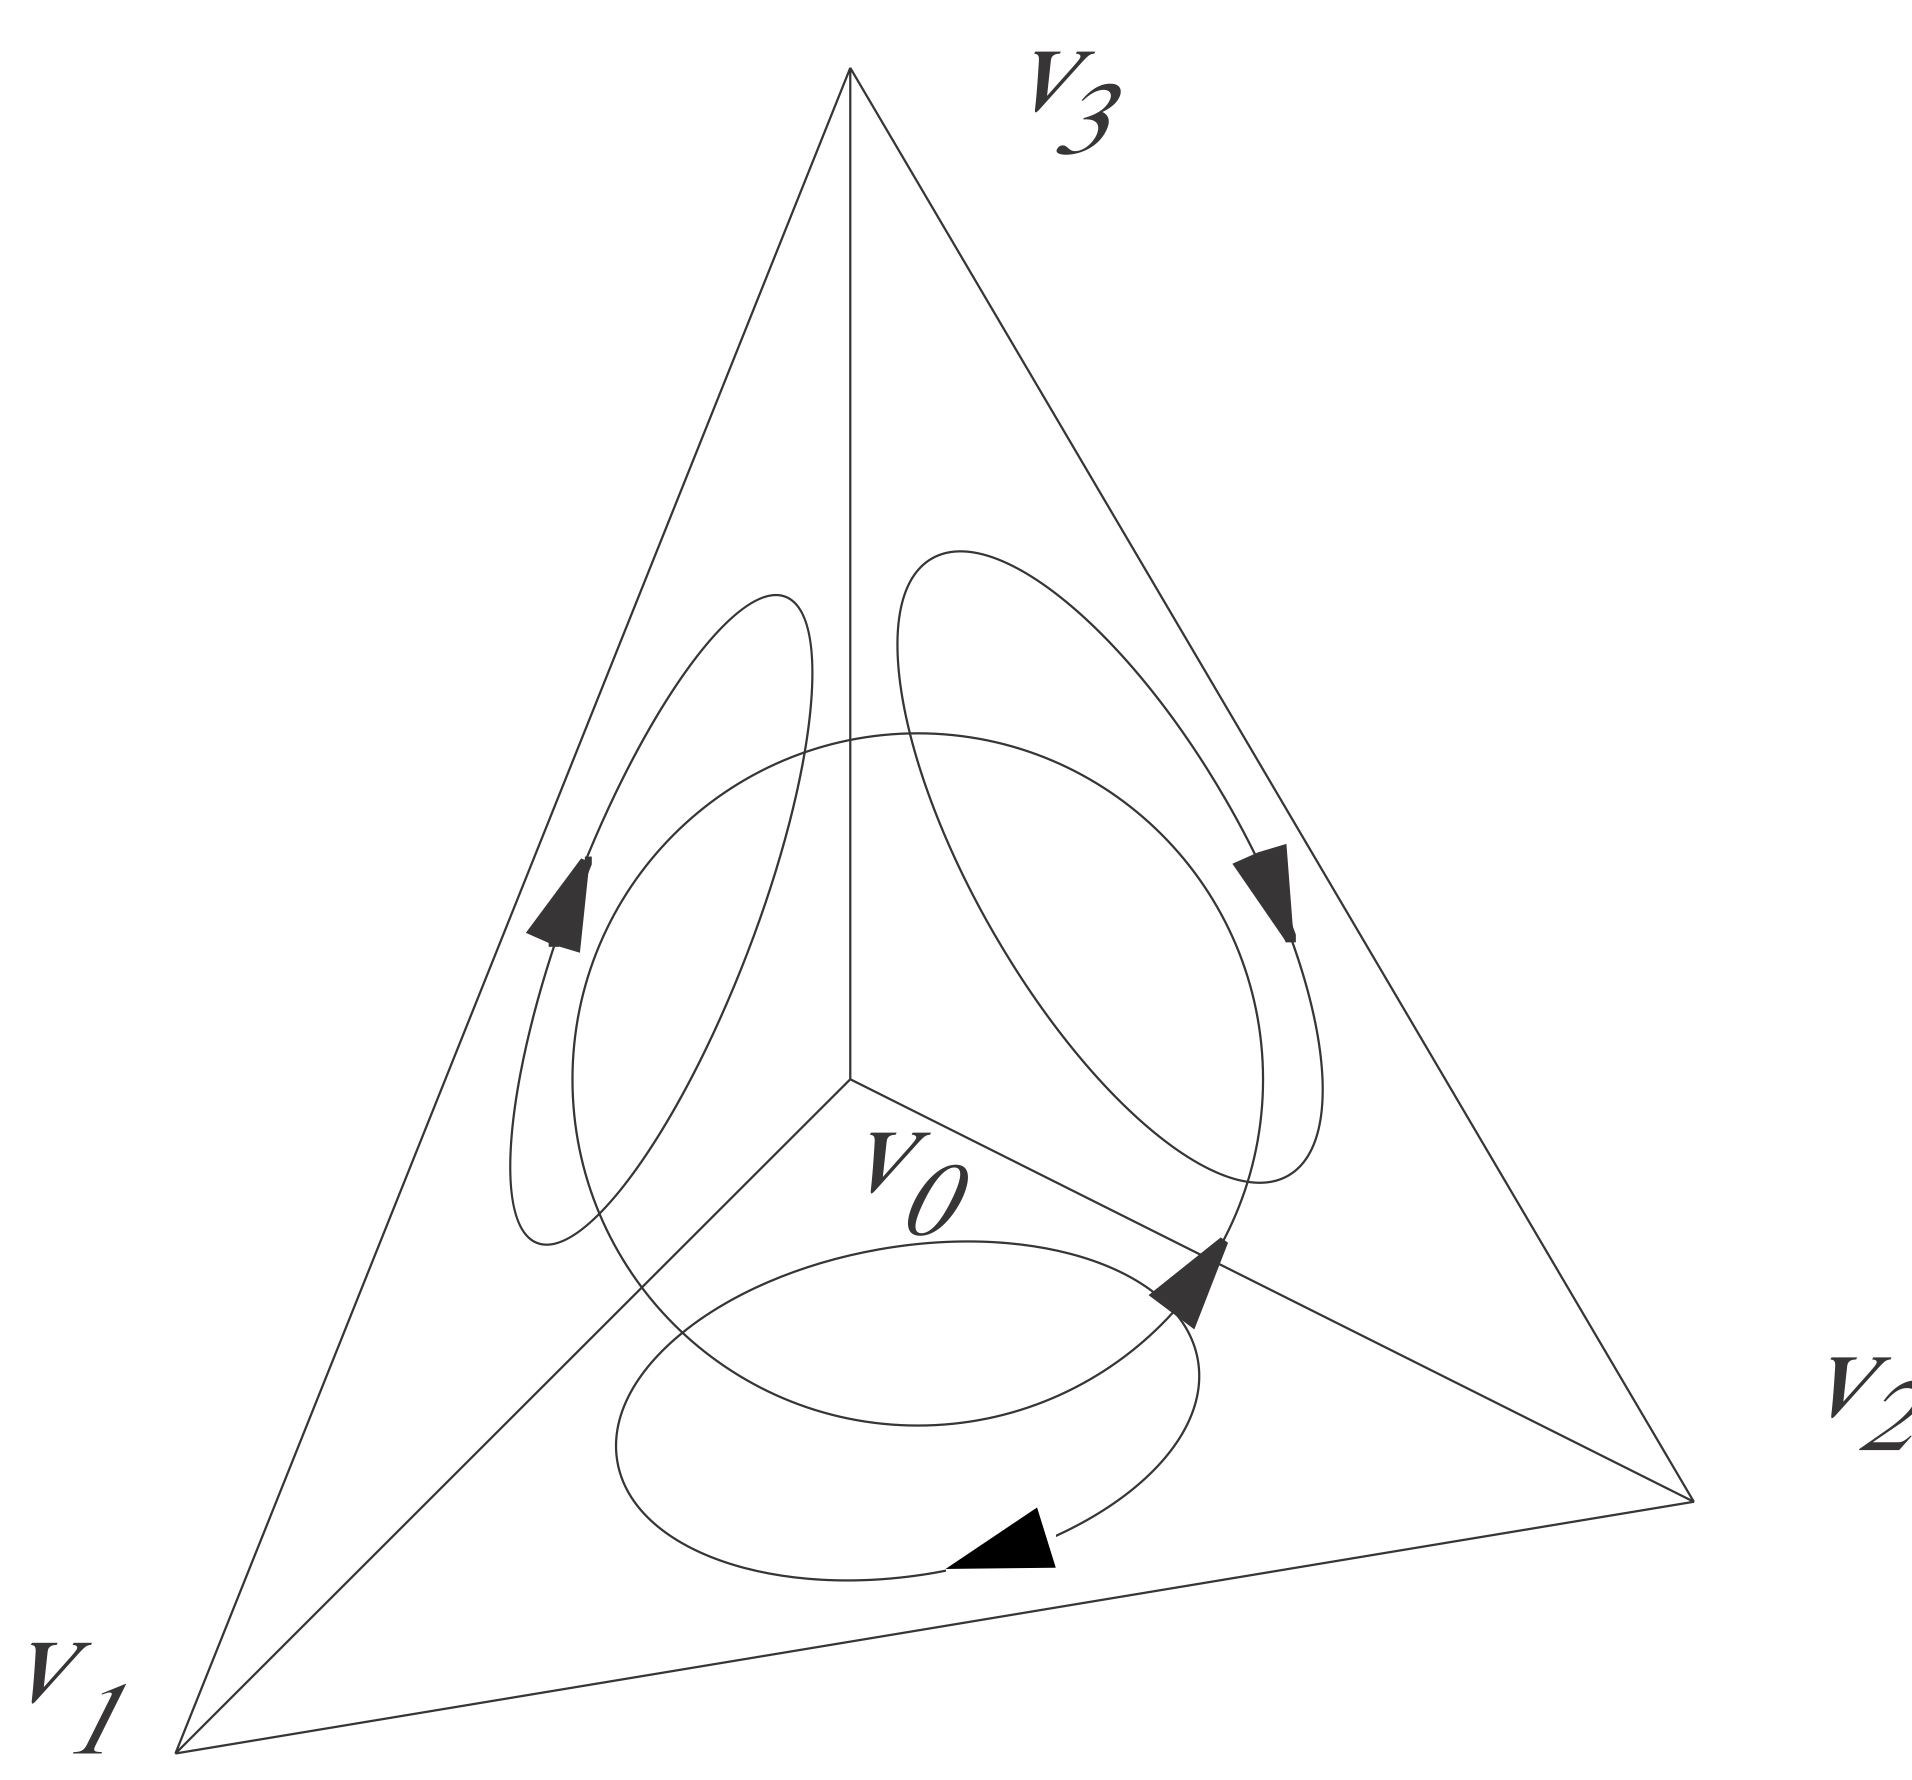
\includegraphics[width=2in]{chapter-03/figs/simplex0.png} \hfill~
\caption{Coherent orientation of the 2-faces of a 3-simplex}
\label{fig:6:simplex}
\end{figure}

\begin{definition}[Volume of a 3-simplex]\label{def:simplexvolume}
The volume of a 3-simplex is a 2-cochain (see Section \ref{sect:3-3}) from the cycle of its 2-faces (boundary triangles) to $\R$.  By definition, a 2-cochain is a map from 2-chains to $\R$.
\end{definition}



\subsubsection*{Facet extraction}\index{Faces!extraction}

The $(d-1)$-faces of a $d$-dimensional simplex or complex are also called \emph{facets} since no ambiguity may arise. It is possible to see \cite{Whitney:1957} what follows:

\begin{theorem}[Whitney, 1957]
The oriented facets $\sigma_{d-1}^{(i)}$ $(0\leq i\leq d)$ of the
oriented $d$-simplex $\sigma_d=+\langle \v{v}_0, \v{v}_1, \ldots,
\v{v}_d \rangle$ are obtained by removing the $i$-th vertex
$\v{v}_{i}$ from the $0$-skeleton of $\sigma_d$:
\begin{equation}
\sigma_{d-1}^{(i)}=(-1)^i(\sigma_d - \langle \v{v}_{i}\rangle), \qquad 0\leq 
i\leq d .
\label{eq:4:eq1}
\end{equation}
\end{theorem}
% where the minus sign denotes a subtraction between $0$-skeletons.

The $0$-skeleton of $\sigma_{d-1,(i)}$ is therefore obtained by removing the 
$i$-th vertex from the $0$-skeleton of $\sigma_{d}$ and either by swapping 
a pair of vertices or, better, by inverting the simplex sign, when $i$ 
is odd.  


\begin{coding}[Facets of a $d$-simplex.] A julia function is given here to compute combinatorially all the oriented facets of a |simplices| arrays of $d$-simplexes. A precondition is that all |Vector{Int64}| in the input sequence have the same length.
\lstinputlisting[language=JuliaLocal,style=julia,mathescape=false]{/Users/paoluzzi/Documents/dev/PLASM/SPRINGER/BOOK/chapter-06/src/009.jl}
If the |expr| after |@assert| is |false|, the program stops in |AssertionError:expr| 
\end{coding}

\begin{coding}[Execution example.] We can start from an array of simplices of the same length and iterate on their facets, to get a whole simplicial complex.
\begin{lstlisting}[language=JuliaLocal, style=julia, mathescape = true]
FV = [[1, 2, 3], [1, 2, 4], [1, 3, 4], [2, 3, 4]] #=
[[1, 2, 3], [1, 2, 4], [1, 3, 4], [2, 3,4]] =#
EV = simplexfacets(FV)  #=
[[1, 2], [1, 3], [1, 4], [2, 3], [2, 4], [3, 4]] =#
VV = simplexfacets(EV)  #=
[[1], [2], [3], [4]]     =#
simplex(3,complex=true).C   #=
Dict(:c1v => EV, :c3v => [[1,2,3,4], :c0v => VV], :c2v => FV) =#
\end{lstlisting}
\end{coding}
We can also generate directly the whole bounday complex of a multidimensional simplex

\begin{coding}[Generation of boundary complex]\ 
We can olso directly generate the |Lar| boundary complex of a simplex of any degree:
\begin{lstlisting}[language=JuliaLocal, style=julia, mathescape = true]
simplex(4,complex=true).C			#=
Dict{Symbol, AbstractArray} with 5 entries:
  :C4V => [[1, 2, 3, 4, 5]]
  :C3V => [[1, 2, 3, 4], [1, 2, 3, 5], [1, 2, 4, 5], [1, 3, 4, 5], [2, 3, 4, 5]]
  :C0V => [[1], [2], [3], [4], [5]]
  :C2V => [[1, 2, 3], [1, 2, 4], [1, 2, 5], [1, 3, 4], [1, 3, 5], [1, 4, 5], [2…
  :C1V => [[1, 2], [1, 3], [1, 4], [1, 5], [2, 3], [2, 4], [2, 5], [3, 4], [3, …  =#
simplex(4,complex=true).V			#=
4×5 Matrix{Float64}:
 0.0  1.0  0.0  0.0  0.0
 0.0  0.0  1.0  0.0  0.0
 0.0  0.0  0.0  1.0  0.0
 0.0  0.0  0.0  0.0  1.0			 =#
\end{lstlisting}
\end{coding}


\begin{coding}[Simplex generation in \texttt{Hpc}]\ 
Convnersely, the |Plasm| data structure |Hpc| contains a single convex cell:
\begin{lstlisting}[language=JuliaLocal, style=julia, mathescape = true]
SIMPLEX(4)			#=
Hpc(MatrixNd(5), Geometry([[0.0, 0.0, 0.0, 0.0], [1.0, 0.0, 0.0, 0.0], [0.0, 1.0, 0.0, 0.0], [0.0, 0.0, 1.0, 0.0], [0.0, 0.0, 0.0, 1.0]], hulls=[[1, 2, 3, 4, 5]]))			 =#
\end{lstlisting}
\end{coding}

\begin{definition}[Simplicial extrusion]

The prism over a simplex $\sigma_{d} = \langle \p{v}_{0},\ldots,
\p{v}_{d} \rangle$, defined as the set $P_{d+1} := \sigma_{d} \times
[a,b]$, with $[a,b]\subset\E$, will be called \emph{simplicial $(d+1)$-prism}. 
An oriented complex which triangulates $P_{d+1}$ can be defined
combinatorially, by using a closed form formula for its ${\cal
K}_{d+1}$ skeleton:
\[
{\cal K}_{d+1} = \{ \sigma_{d+1,(i)} = (-1)^{id}
\langle \p{v}_{i}^{a},\p{v}_{i+1}^{a},\ldots,\p{v}_{d}^{a},
\p{v}_{0}^b,\p{v}_{1}^b,\ldots,\p{v}_{i}^b \rangle, \quad  0\leq i\leq d \}
\]
where $\p{v}_{i}^{a} = (\p{v}_{i},{a})$ and $\p{v}_{i}^{b} = 
(\p{v}_{i},{b})$.

Closed formulas to triangulate the $(d+1)$-prism over a $d$-complex in
a time linear with the size of the output, while computing also the
$d$-adjacencies between the resulting $(d+1)$-simplices, can be found
in~\cite{10.1016/0010-4485(91)90080-G,10.1145/164360.164376}.
\end{definition}


\subsection*{Simplicial grids}\index{Linear!d-Polyhedra}

In layout design, a grid system provides a framework of intersecting vertical and horizontal lines. Designers use this framework to place and align text, images, and other elements. 

Analogously, a \emph{simplicial grid}, is a geometric grid structure made by simplicial cells of same dimension aligned on a layout grid 1D, 2D, 3D, etc.
They are mainly used for domain decomposition, where to map coordinate functions in order to create curved structures, i.e., proper curves, curved surfaces, and curved solids.

The whole curved complex is easily generated by mapping the vertices of a |Lar| grid.


\begin{figure}[] %  figure placement: here, top, bottom, or page
   \centering   
   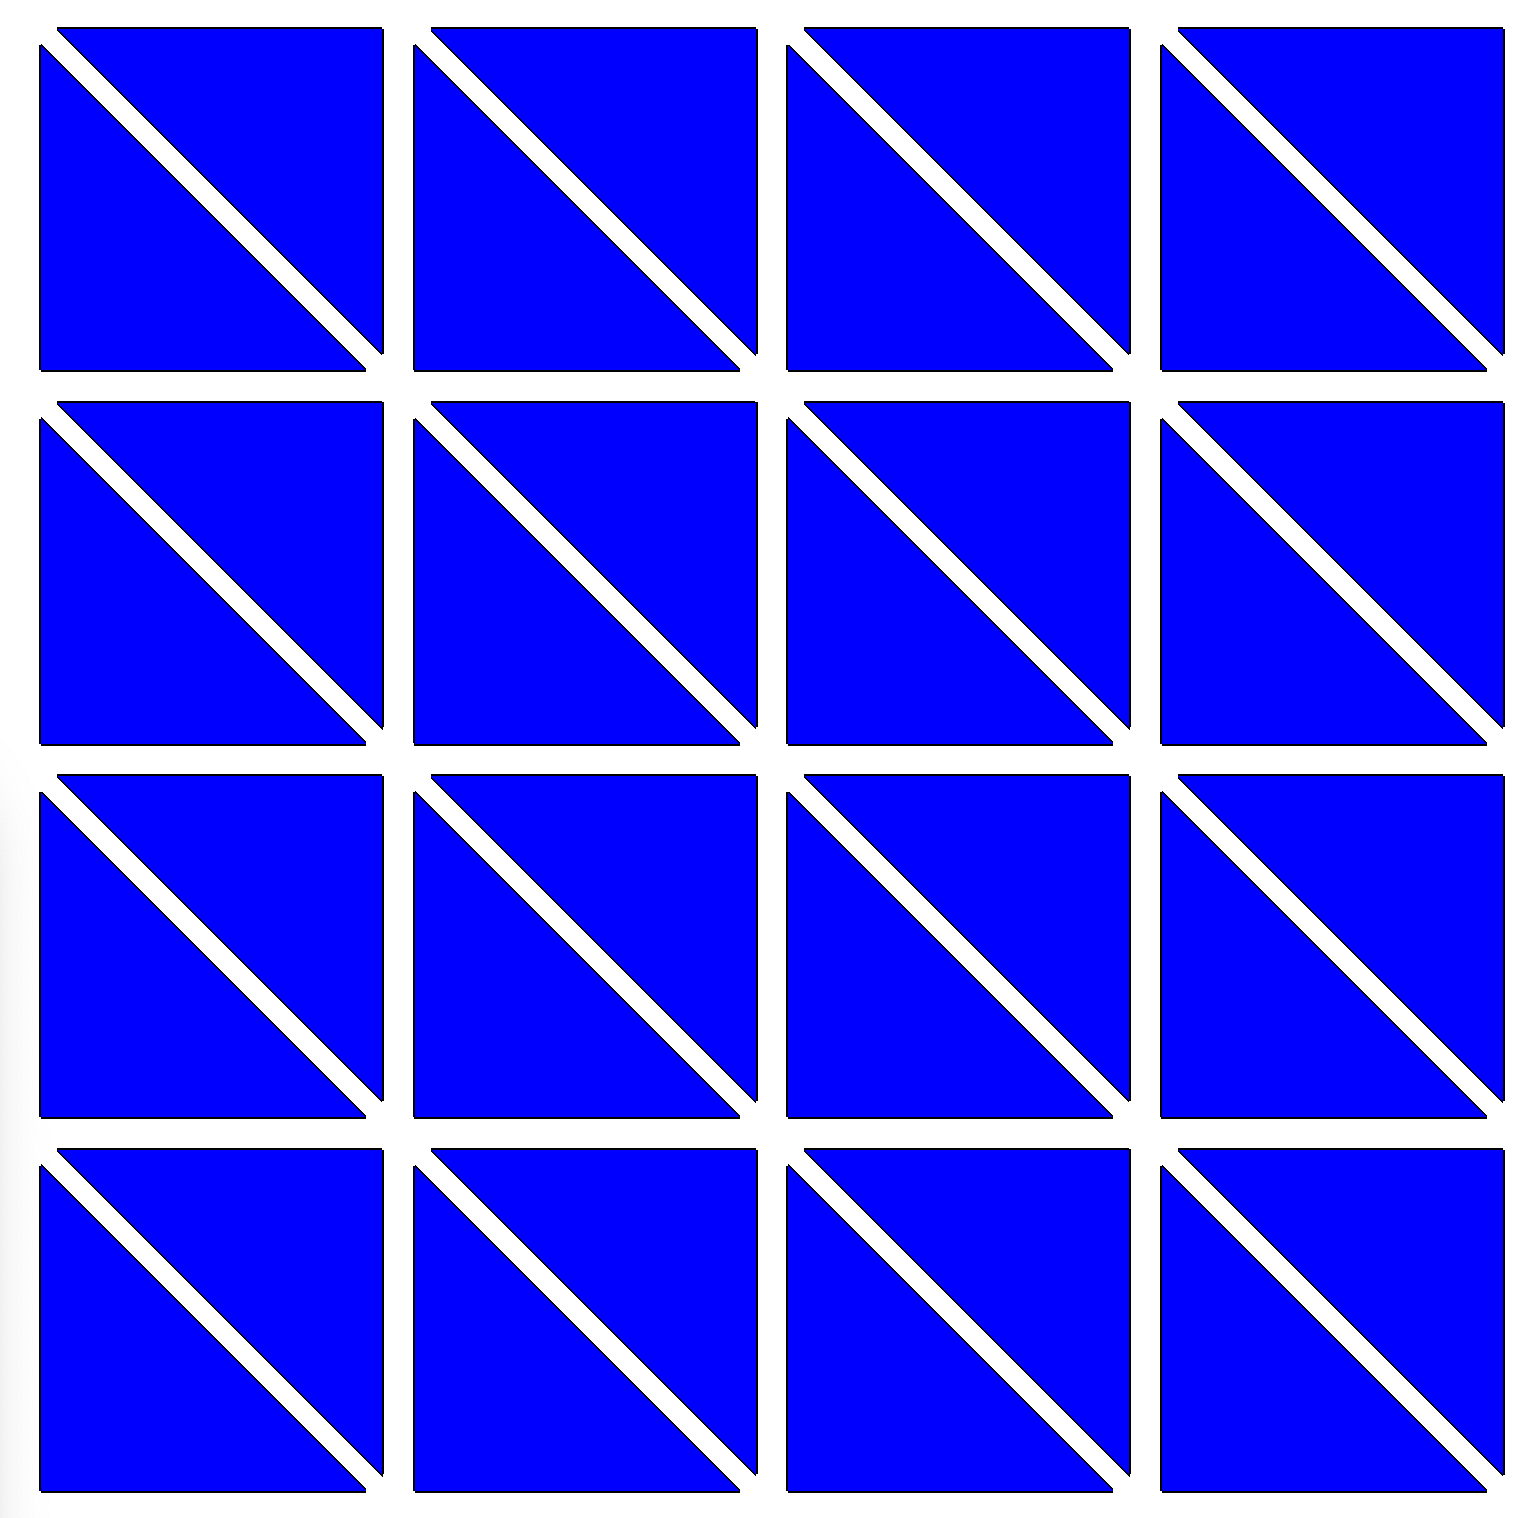
\includegraphics[width=0.29\textwidth]{chapter-03/figs/extrude02.png}% 
   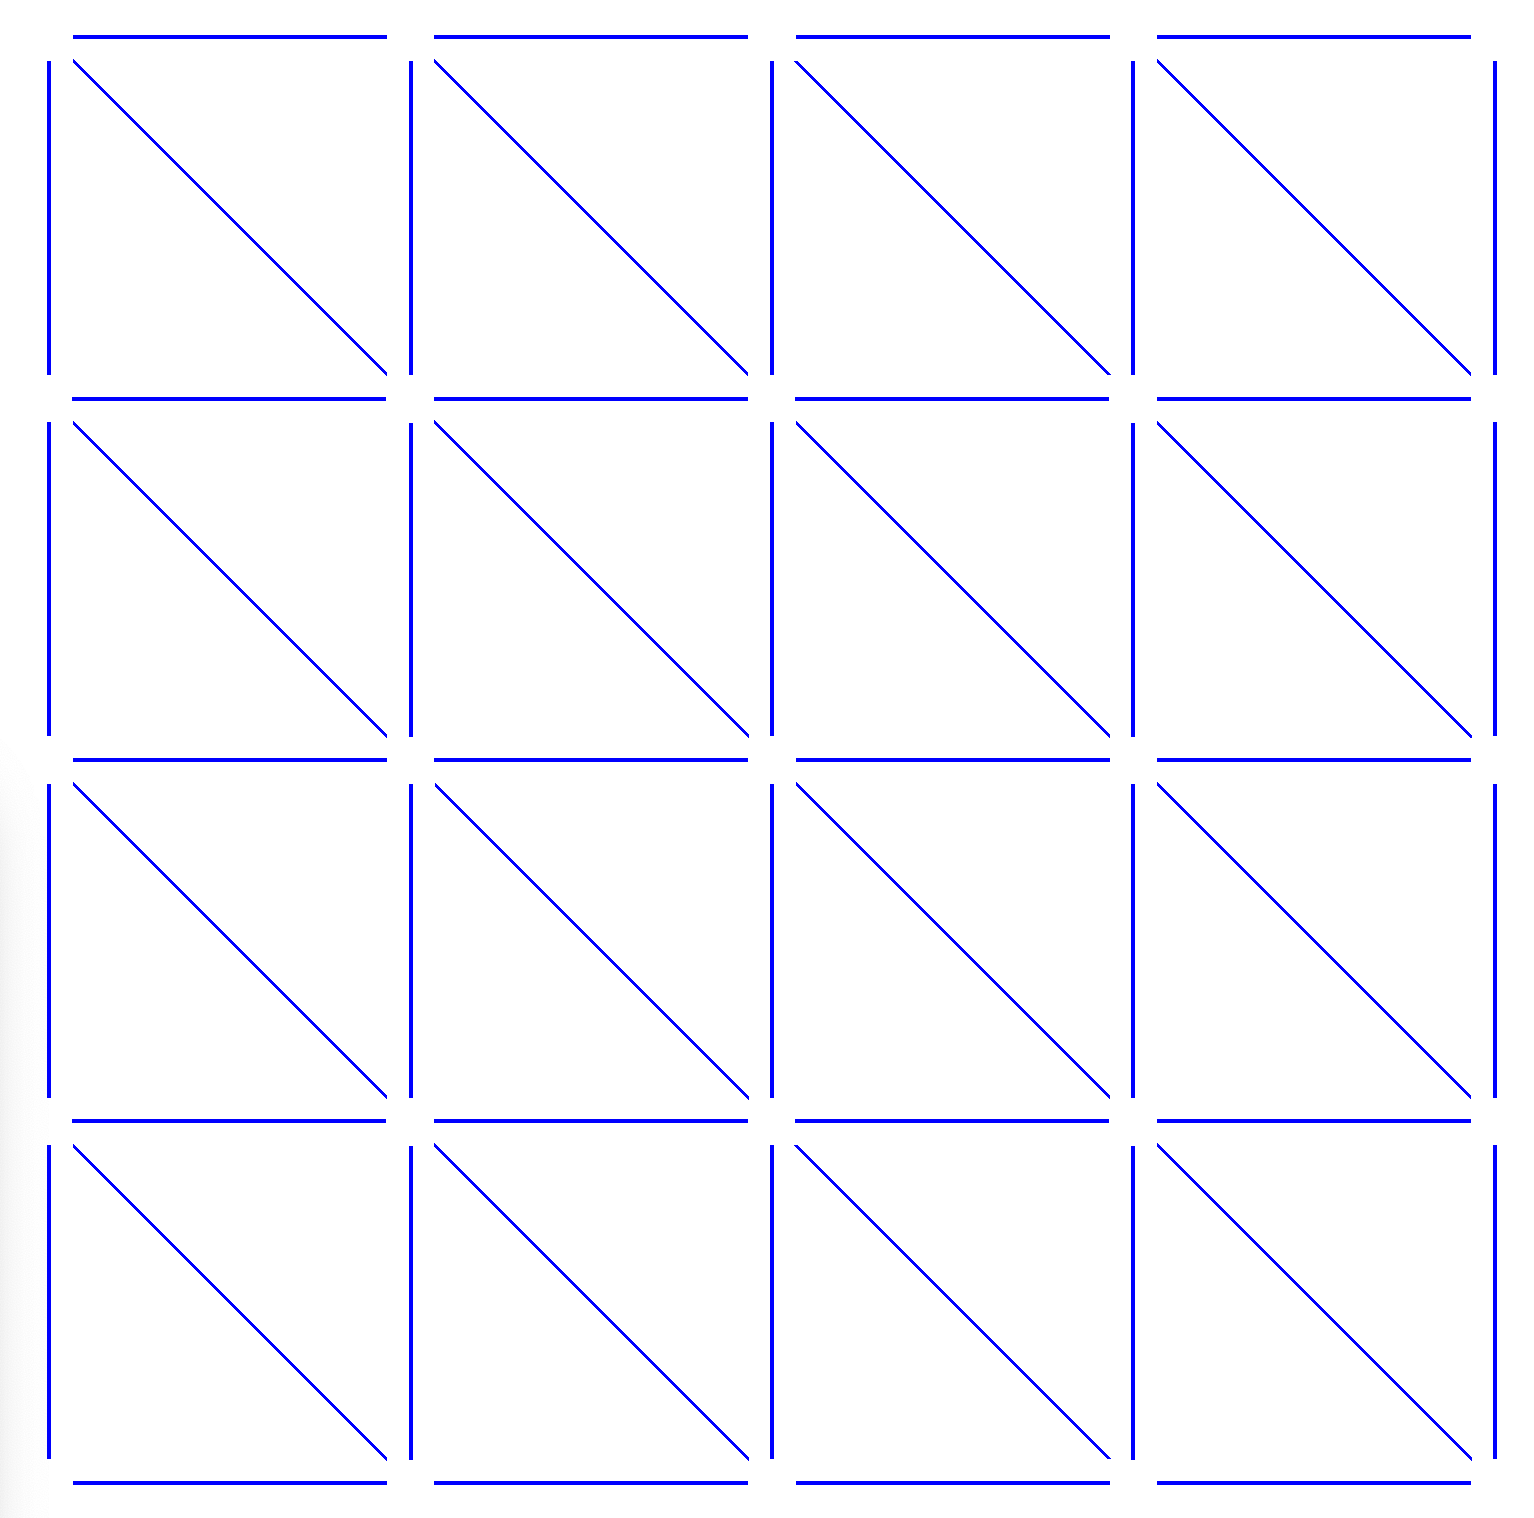
\includegraphics[width=0.29\textwidth]{chapter-03/figs/extrude03.png} 
   \caption{The simplicial 2- and 1-complex (shown here slightly exploded) are generated by \emph{extrudecomplex()} using the same pattern, both starting from \emph{model1D}.
   The 1-complex is derived by the 2-complex using \emph{simplexfacets()}.}
   \label{fig:3:extrude1}
\end{figure}

\begin{coding}[1D Extrusion]\ 
\begin{lstlisting}[language=JuliaLocal, style=julia, mathescape=false]
V1 = [ 0.0 1.0 2.0 3.0 4.0 5.0 ]
EV = [[1, 2], [2, 3], [3, 4], [4, 5]]
mod1D = Lar(V1, Dict(:c1v => EV))
V2 = [mod1D.V; zeros(size(mod1D.V,2))']
GL.VIEW(GL.GLExplode(V2, map(x->[x],EV),1.1,1.1,1.1,2,1));
\end{lstlisting}
\end{coding}

The |mod2D| and |mod3D| grids are generated by the following code.

\begin{coding}[2D Extrusion]\
\begin{lstlisting}[language=JuliaLocal, style=julia, mathescape=false]
mod2D = extrudecomplex(mod1D::Lar, [1, 1, 1, 1])
FV = collect(values(mod2D.C))[1]
EV = simplexfacets(FV)
GL.VIEW(GL.GLExplode(mod2D.V, map(x->[x],EV),1.2,1.2,1.2,4,1));
\end{lstlisting}
\end{coding}

\begin{coding}[3D Extrusion]\
\begin{lstlisting}[language=JuliaLocal, style=julia, mathescape=false]
mod3D = extrudecomplex(mod2D::Lar, [1,-2,1])
CV = collect(values(mod3D.C))[1]
FV = simplexfacets(CV)
EV = simplexfacets(FV)
GL.VIEW(GL.GLExplode(mod3D.V,map(x->[x],EV),2,2,2,99,1));
\end{lstlisting}
\end{coding}

\begin{figure}[] %  figure placement: here, top, bottom, or page
   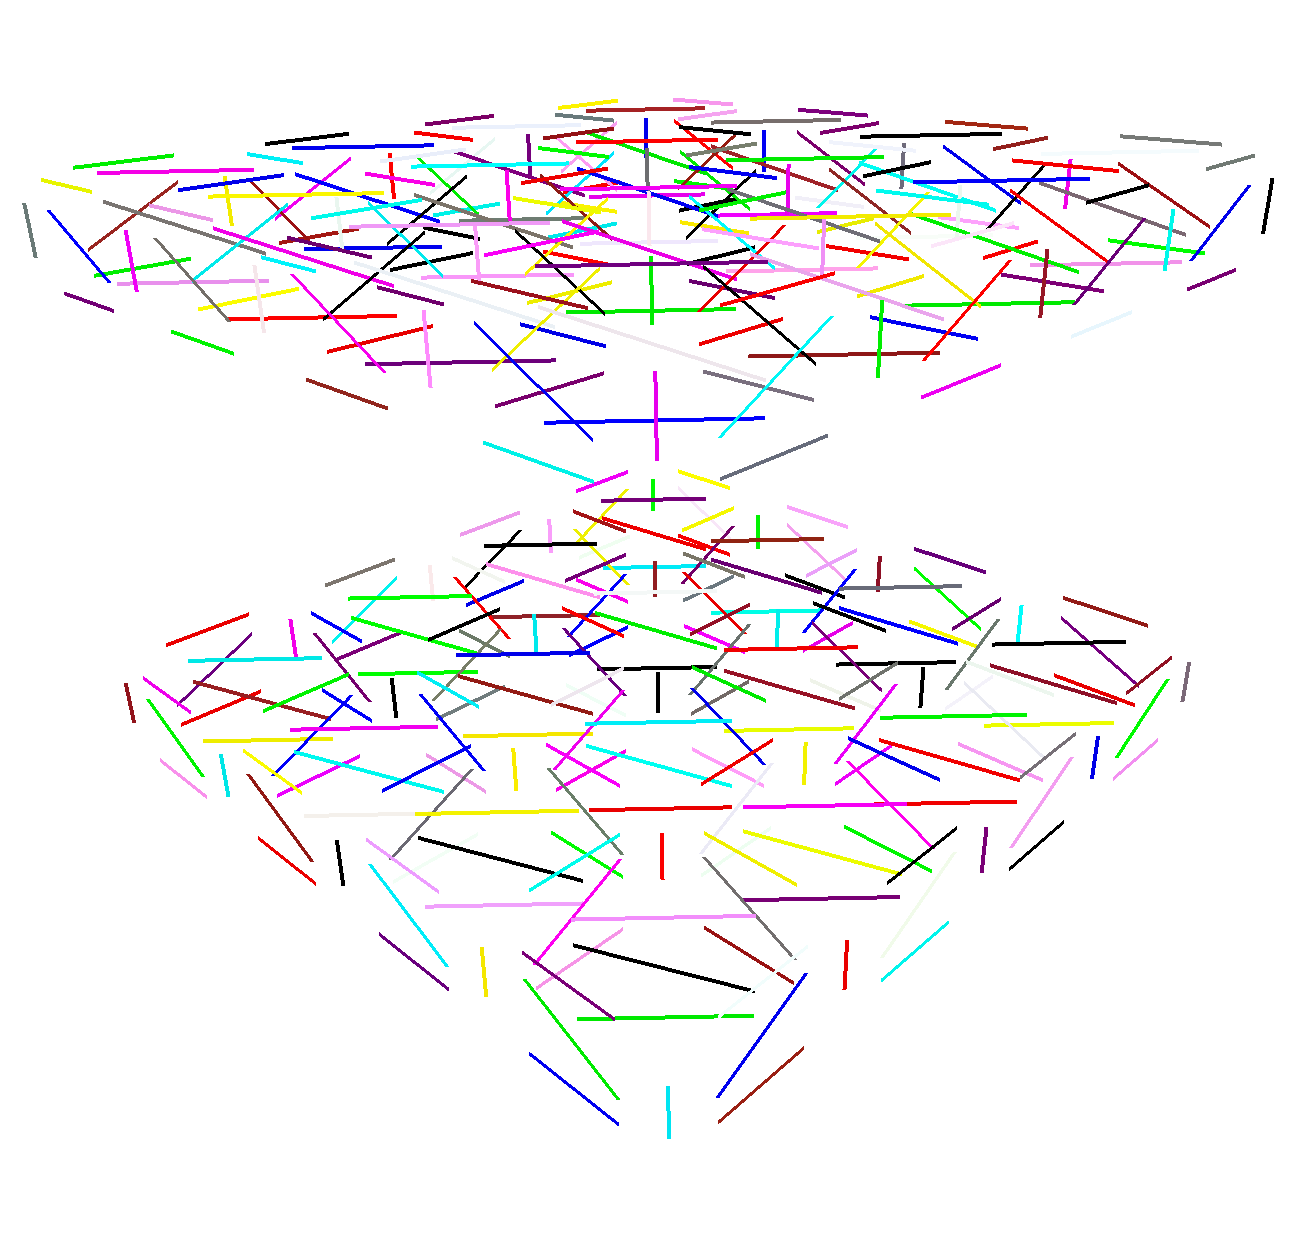
\includegraphics[eight=0.335\linewidth,width=0.33\linewidth]{chapter-03/figs/extrude06.png}%
   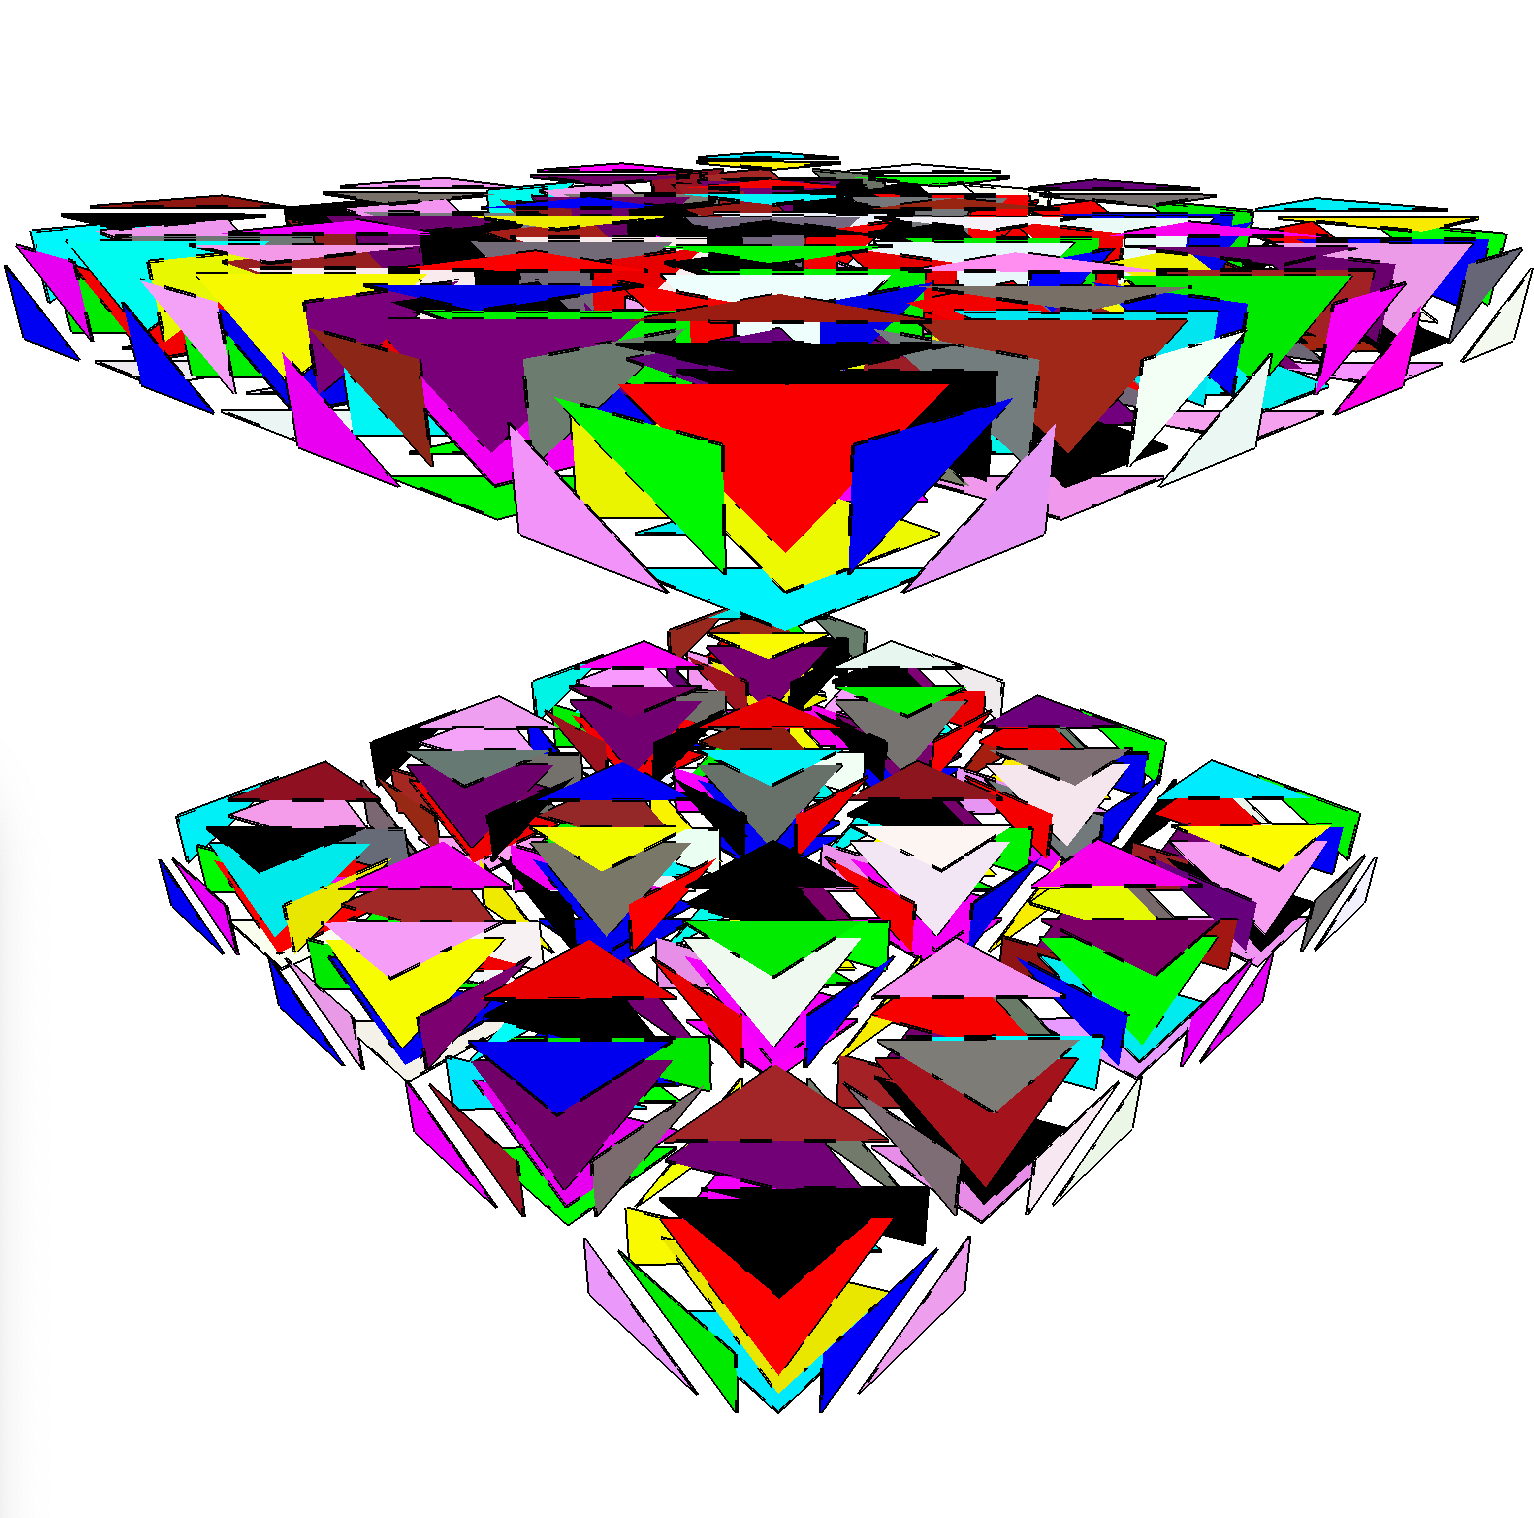
\includegraphics[eight=0.33\linewidth,width=0.33\linewidth]{chapter-03/figs/extrude04.png}%
   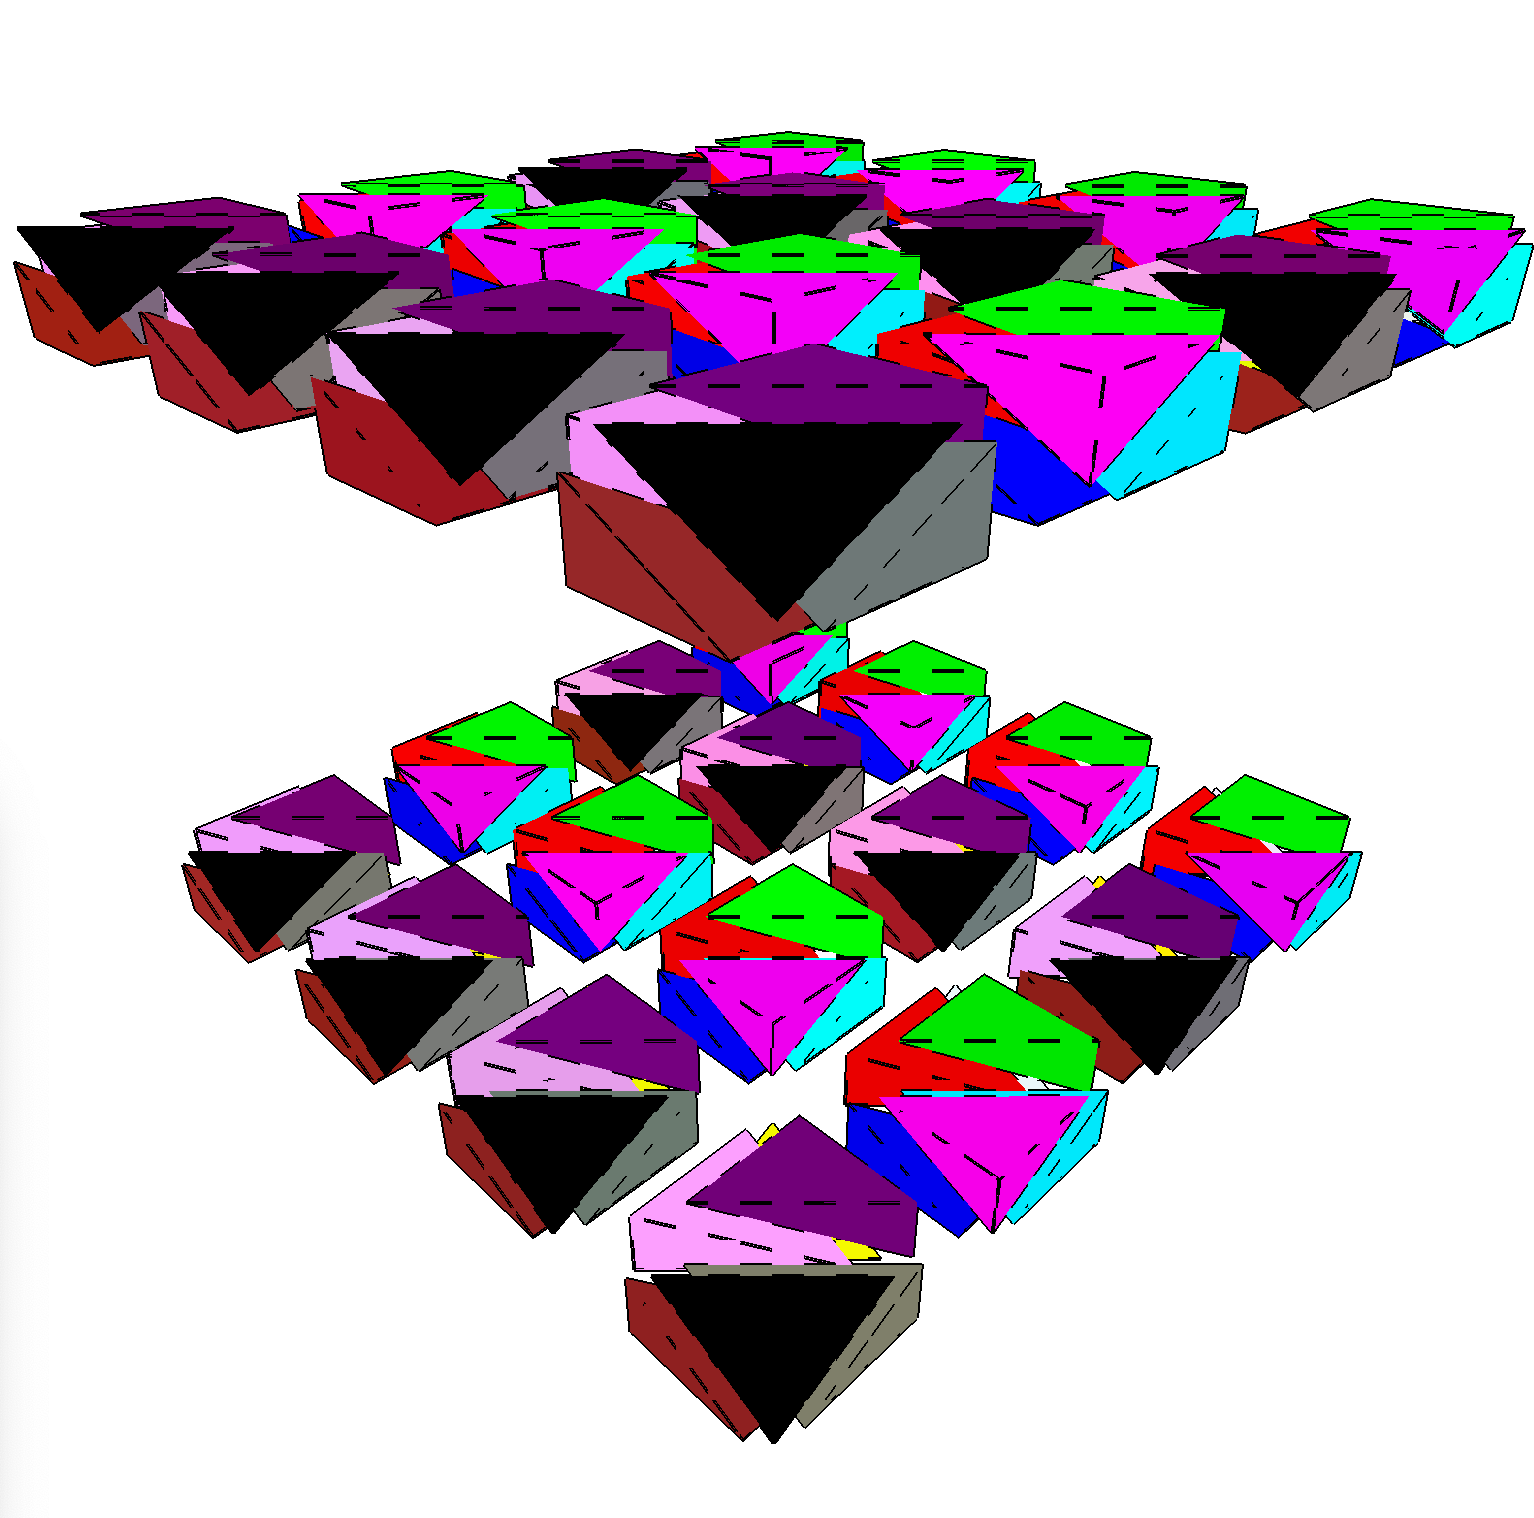
\includegraphics[eight=0.33\linewidth,width=0.33\linewidth]{chapter-03/figs/extrude05.png}\hfill
   \caption{Exploded simplicial grids of dimensions 1 (lines), 2 (surfaces), and 3 (solids). The simplicial 2-complex is generated by \emph{simplexfacets()} from the 3-complex \emph{extrudecomplex(simplex2D)}, with \emph{simplex2D} in turn starting from \emph{model1D}, i.e., from the expression generating the simplicial 1-complex \inlinegraphics{chapter-03/figs/complex1D.png}. }
   \label{fig:3:extrude2}
\end{figure}



\subsection{Cubical complex and grid}\label{sect:3-2-2}


We introduce now the definition and use of multidimensional \emph{grids} of \emph{cuboidal}, and the more general \emph{Cartesian product} of cellular complexes. Such operators, depending on the dimension of their input, may generate either \emph{full-dimensional} (i.e. solid) output complexes, or \emph{lower-dimensional} complexes of dimension $d$ embedded in Euclidean $n$-space, with $d\leq n$.  

\subsubsection*{Regular grid}


Regular cubical grids appear in finite element analysis, finite volume methods, finite difference methods, and in general for discretization of parameter spaces. 

\begin{definition}[Regular cuboidal grid] A regular grid is a tessellation of n-dimensional Euclidean space by congruent parallelotopes (e.g. bricks). Its opposite is irregular grid. We prefer to call these objects “cuboidal” complexes, in order to remark their multidimensional character in |Plasm|.
\end{definition}


\begin{figure}[] %  figure placement: here, top, bottom, or page
   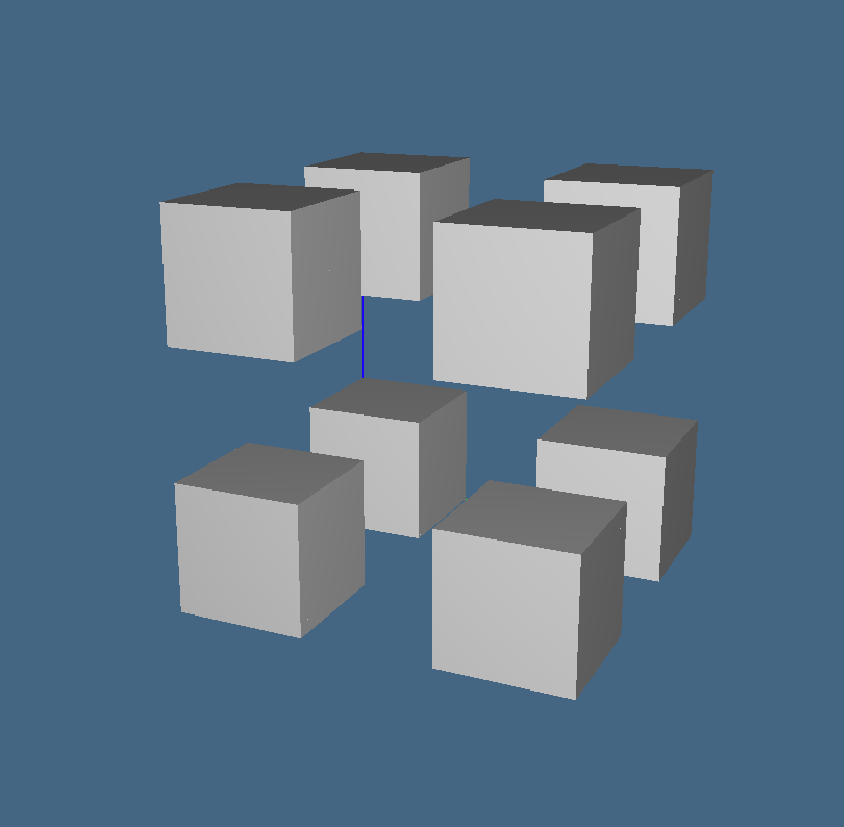
\includegraphics[height=0.5\linewidth,width=0.5\linewidth]{chapter-03/figs/cubic01}%
   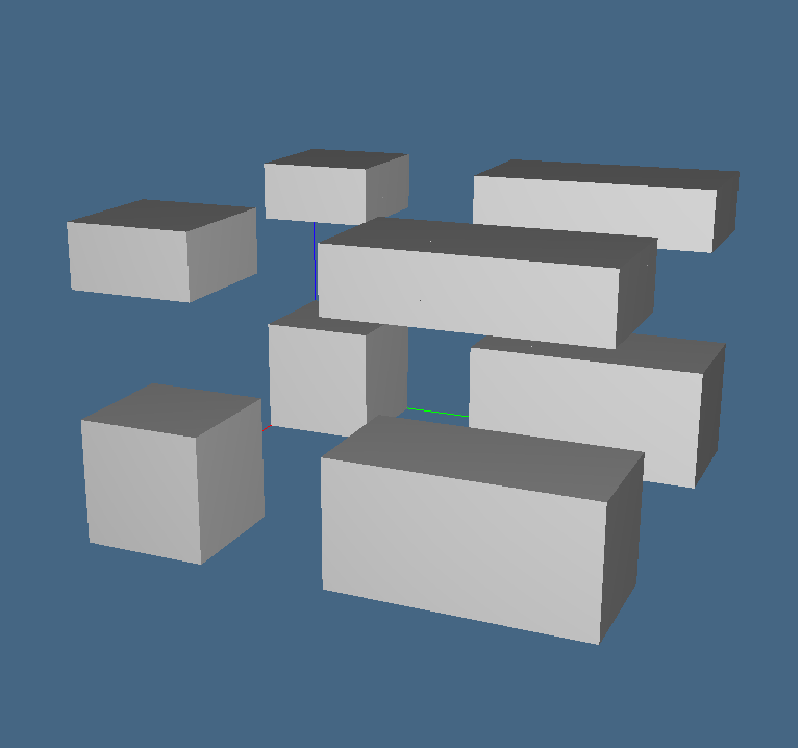
\includegraphics[height=0.5\linewidth,width=0.5\linewidth]{chapter-03/figs/cubic02}%
   \caption{Unconnected cubical grids: (a) regular cell complex; (b) irregular cell complex. See Script~\ref{script-3.2.12}.}
   \label{fig:3:cubics}
\end{figure}


E.g., just think to a mesh of 3D cubes in three-dimensional space for the first case, and to the (non-manifold) framework of skeletal polygons of such cubic cells for the second case.

In particular,  both $n$-dimensional \emph{solid grids} of (hyper)-cuboidal cells and their  $d$-dimensional \emph{skeletons} ($0\leq d\leq n$), embedded in $\E^n$, are generated by assembling the cells produced by a product of $n$ either 0D or 1D cellular complexes, that in such lowest dimensions coincide with {simplicial complexes}. 

In |Plasm| the cuboidal grids are not necessarily regular, and can be even unconnected. 

\begin{coding}[3D Cell Complex]\label{script-3.2.12}
Two simple examples  of 3D  cuboidal grids are shown in Figure~\ref{fig:3:cubics}. Each |GRID| instance generates a 1D cellular complex, and two Cartesian product, denoted in |Plasm| by the |*| infix symbol, produce the 3D cell complex.
\begin{lstlisting}[language=JuliaLocal, style=julia, mathescape=false]
VIEW(GRID([1,-1,1]) * GRID([1,-1,1]) * GRID([1,-1,1]))
VIEW(GRID([1,-2,1]) * GRID([1,-1,2]) * GRID([1,-1,0.5]))
\end{lstlisting}
It is easy to believe that negative parameters denote empty space, while the positive ones denote full space. See Figure~\ref{fig:3:cubics}.
\end{coding}







\subsection{Polyhedral complex}\label{sect:3-2-3}


\subsection*{Topological product}
\label{subsec:2:style}

In this section, we discuss a solid modeling operation highly useful to generate 3D solids from 2D surfaces, as well as 2-complexes from 1-complexes, and to produce their skeletons taking advantage of one or more 0-complexes.

\begin{definition}[Topological product]
A product space is the \emph{Cartesian product} of a family of topological spaces equipped with a natural topology.
\end{definition}

The natural topology on a subset of a topological space, in our case $\E^d$, is the relative topology (or subspace topology).
The product of two cell complexes can be made into a cell complex as we show in the following. 

\begin{definition}[Product of cell complexes]
If $X$ and $Y$ are  $m$- and $n$-complexes in $\E^m$ and $\E^n$, respectively,  $X \times Y \subset \E^{m+n}$ is a cell complex in which each cell is a product of a cell in $X$ and a cell in $Y$, endowed with the relative topology in $\E^{m+n}$.
\end{definition}

\subsection*{Cell complex product}
\label{subsec:6:cell-product}

\begin{definition}[larprod]
The |Plasm| |POWER| function, also denoted as infix |*|, takes as input a pair of |Plasm| models of |Hpc| type, and returns the value |Hpc| of their \emph{Cartesian product}. 
\end{definition}
The operation is associative, hence no parenthesis are needed, as you can see in Coding~\ref{script-3.2.12}.



\section{Chain complex}\label{sect:3-3}

This section deals with algebraic topological tools to compute boundaries and adjacencies of \emph{chains} of cells, and  to generate the discrete solid primitives needed by a  computational modeler. 
Basic geometric and algebraic topology  
provide the mathematical concepts needed to compute
and explore the cells of the space partition induced by a set of
geometric objects, as well as the related incidence/neighborhood relations. 

%To our knowledge, algorithms for computing with chain complexes  only include  the recent paper~\cite{Alayrangues2015}, where combinatorial generalized maps~\cite{Lienhardt:2014}, a quite intricate data structure, are used for cycles/boundary calculation of the homology of a cellular complex.  Conversely, it is well known~\cite{Munkres:84,Kannan:79,Paoluzzi:1993:DMS:169728.169719,Edelsbrunner:95} that for simplicial  complexes---\emph{aka} well-formed triangulations---boundary operators are defined as linear extensions of basic boundary operators which act on simplices. 

To work over huge geometric datasets we need explicit expression of topological relations using proper and efficient computational structures.
The purpose of this chapter is to elucidate our best methods for multidimensional solid modeling computing.
The geometric discussion is restricted to piecewise-linear topology and to space dimensions less or equal to three.

Some words about  notations:  greek letters are used for the \emph{cells} of a space partition, and roman letters for  \emph{chains} of cells, coded in coordinates as either signed integers or sparse arrays of signed integers.  


\subsection{Linear chain spaces}\label{sect:3-3-1}

In mathematics, a graded vector space is a vector space that has the extra structure of a gradation, which is a decomposition of the space into a direct sum of vector subspaces, generally indexed by the integers.

\begin{definition}[Graded vector space]\label{def:3:graded}
A \emph{graded vector space} is a vector space $V$ expressed as a direct sum  of
subspaces $V_p$ indexed by integers in $[0,d] := \{p\in\N \ :\ 0\leq p\leq d\}$:
\begin{equation} 
V = \oplus_{p = 0}^d V_p.
\end{equation} 
\end{definition}

\begin{definition}[Graded linear maps]\label{def:graded}
A linear map $f:V\to W$ between graded vector spaces is a \emph{graded
map} of degree $k\ $ if $f(V_p) \subset W_{p+k}$ for each $p$.
\end{definition}

Let be given a cellular complex $X$. We are interested in working with subsets of cells with the \emph{same} dimension, and with their 1-graded maps, which completely specify the $X$ topology.

\begin{definition}[$p$-chain]
A \emph{$p$-chain} can be seen, with some abuse of language, as \emph{any subset} of $p$-cells in a cellular complex $X$. 
\end{definition}


\begin{definition}[Unit $p$-chain]
In this sense we write $U_p = \Lambda_p - \Lambda_{p-1}$ for the set of \emph{unit} (or \emph{elementary}) $p$-chains ($0\leq p\leq d$), where $\Lambda_p$ is the $p$-skeleton of $X$ and $\Lambda_{-1} = \emptyset$.
\end{definition}

\begin{definition}[Linear $p$-space]
$C_p = \mathcal{P}(U_p)$ is the space of $p$-chains, where $\mathcal{P}$ is the power set.
\end{definition}

The set $C=\oplus\ C_p$, direct sum of chain spaces, can be given the structure of a graded vector space (see \ref{def:3:graded} and \cite{Arnold:2018}) by
defining sums of chains with the same dimension, and products times scalars in a
field, with the usual properties.
%\end{definition}

\begin{definition}[Chain bases]
As a linear space, each $C_p$ contains a set of irreducible generators.
The natural \emph{basis} $U_p \subset C_p$  is the set of \emph{independent} (or \emph{elementary}) chains $u_p \in C_p$, given
by singleton elements. Consequently, every chain $c\in C_p$ can be written as 
a linear combination of this basis with field elements, and is uniquely generated. 
\end{definition}

Once  the  basis is fixed, \emph{i.e.}, $U_p$ is ordered, the unique unsigned coordinate
representation of each $\{\lambda_k\} =: u_k \in C_p$ is a binary array with one non-zero element in position $k$, and all other elements 0. The ordered
sequence of scalars may be drawn either from $\{0,1\}$ (unsigned representation) or from
$\{0,1,-1\}$ (oriented representation). 
With abuse of language, we
often call $p$-cells the elements of $U_p$.
%\end{definition}


\begin{definition}[Chain complex]
A \emph{chain complex} is a graded vector  space $V$ provided with a graded
linear map $\partial : V \to V$ of degree $-1$ called
\emph{boundary operator}, which satisfies $\partial^2 = 0$. 
\end{definition}


In other words, a chain complex
is a sequence of vector spaces $C_p$ and linear maps $\partial_p : C_p \to C_{p-1}$,
such that $\partial_{p-1} \circ\ \partial_{p} = 0$. \rtwocol{The notation $C_\bullet$ is used in this paper for the chain complex over the binary field $\{0,1\}$, and ${C}^\circlearrowleft_\bullet$ for the oriented chain complex over the ternary field $\{0,1,-1\}$, used to get oriented boundaries. 
}


\begin{definition}[Cochain complex]
A \emph{cochain complex} is a graded vector space $V$ furnished with a graded
linear map $\delta : V \to V$ of degree $+1$ 
called \emph{coboundary operator},  which satisfies $\delta^2 = 0$. 
\end{definition}

That is to say, a cochain complex is a
sequence of vector spaces $C^p$ and linear maps $\delta^p : C^p \to C^{p+1}$,
such that $\delta^{p+1} \circ\ \delta^{p} = 0$. 

\begin{remark}
The reader should note, as rule of dumb to remember the meaning of boundary and coboundary operators, that boundaries map cells in decreasing dimensions, and coboundaries in increasing dimensions. So, e.g., it is $\partial_2: C_2\to C_1$ and $\delta_1: C_1\to C_2$. Note also that every operator index is the one of its domain.
\end{remark}


\subsection{Linear chain operators}\label{sect:3-3-2}

\begin{definition}[Chain complex]
A \emph{chain complex} is a sequence of linear spaces \(C_p\) of chains and linear
boundary/coboundary maps \(\partial_p, \delta_p\) between them: 
\end{definition}
Given a collection \(\mathit{S}\) of geometric
objects\footnote{Examples include, but are not limited to: line segments, quads, triangles, polygons, meshes, pixels, voxels, volume images, B-reps, \emph{etc.} 
In mathematical terms, a geometric object is a topological space embedded in some $\E^d$ \cite{Edelsbrunner:95}.},
we shall compute the topology of their space
arrangement \(\mathcal{A}(\mathit{S})\) as a chain complex (see Section~\ref{chapt:7})

\[ 
C_\bullet = (C_p, \partial_p) := 
C_3 \ 
\substack{
\delta_2 \\
\longleftarrow \\[-1mm]
\longrightarrow \\
\partial_3 
}
\ C_2 \ 
\substack{
\delta_1 \\
\longleftarrow \\[-1mm]
\longrightarrow \\
\partial_2 
}
\ C_1 \ 
\substack{
\delta_0 \\
\longleftarrow \\[-1mm]
\longrightarrow \\
\partial_1 
}
\ C_0\ ;\] 
\[
\delta_p=\partial_{p+1}^\top\qquad 3\leq p\leq 0
\]





{In the remainder of this book we identify chains  and cochains, as in \cite{PAOLUZZI2023103436}.
In this way we express to be only interested to combinatorial topology aspects of cell complexes, and not in differential ones. 

A standard basis, also called a natural basis, is a special orthonormal vector basis in which each basis vector has a single nonzero entry with value 1~\cite{Wolfram:algebra:StandardBasis}.
Being only interested in topological properties, we have identified elementwise the natural bases of the corresponding chain and cochain spaces. 

As a consequence, the boundary and coboundary matrices are related by transposition, and given the coordinate vector of a $p$-cell, provide both the incident $p-1$ and $p+1$ cells, respectively.



\subsubsection*{Operator matrices}

The matrices of boundary and coboundary operators (their transpose) are very
sparse, with sparsity growing linearly with the number $n$ of rows (sparse columns in Julia).  With common data structures~\cite{coosparse} for sparse matrices, 
the storage cost $O(n)$ is linear with the number of cells, with $O(1)$ small cost per cell  that depends on the storage scheme.
\begin{remark}
The standard notation of matrices of operators is given by the operator symbol enclosed between squared brackets. For example $[\partial_3]$ and $[\delta_2]$ stand for the matrices of 3-boundary and 2-coboundary, respectively.\\
\begin{end}

According to what discussed in Section~\ref{sect:3-3-2}, we may identify the $U_0$ basis of 0-chains with the ordered sequence |V| of vertices (0-cells) of a cellular complex, and the $U_1, U_2$ bases of 1- and 2-chains with ordered sequences |E| of edges (1-cells) and |F| of faces (2-cells), respectively. Analogously, we use the symbol |C| for the ordered 3-cells. 

The natural bases of cells remain identified by ordinal numbers of their cells ($1$, $2$, $3$, $\ldots$), and the chain spaces dimension (for example $\dim$ V) by |$\#$V|, |$\#$E|, |$\#$F|, and |$\#$C|.

Therefore, we adopt a pair of characters from $\{$|V|, |E|, |F|, |C|$\}$, for instance |EF|, to denote the matrix of mapping |F|${}\to{}$|E| from 2-chains in |F| to 1-chains in |E|,  in mathematical terms $\partial_2 : C_2 \to C_1$ (see Section~\ref{}).
Hence, for sake of readiness and simplicity we will often use the notations:

\begin{lstlisting}[language=JuliaLocal, style=julia, mathescape = true]
$\delta_2: C_2\to C_3 \equiv\ $CF: F $\to$ C $;\qquad$ $\delta_1: C_1\to C_2 \equiv\ $FE: E $\to$ F $;\qquad$ $\delta_0: C_0\to C_1 \equiv\ $EV: V $\to$ E $.$
\end{lstlisting}

\begin{lstlisting}[language=JuliaLocal, style=julia, mathescape = true]
$\partial_3: C_3\to C_2 \equiv\ $FC: C $;\to$ F $;\qquad$ $\partial_2: C_2\to C_1 \equiv\ $EF: F $\to$ E $;\qquad$ $\partial_1 : C_1\to C_0\equiv\ $VE: E $\to$ V $.$  
\end{lstlisting}

\begin{remark}[Matrix and vector formats]
Actual content of vectors |V,E,F,C| is the coordinate representation of a chain (subset) of topological entities, hence the characteristic function of such subset of cells  (binary vector).
\end{remark}

\begin{remark}[Linear operator vs matrix]
Linear operators between chain spaces work between two linear spaces. The actual application of operator’s matrix produces a range’s vector from a domain’s vector (both in coordinates). Actually, any column of the matrix is one element of domain’s basis  expressed in coordinates of the target space, i.e. by the coefficients of linear combination of the target’s basis.
\end{remark}


\subsubsection*{Matrix-Vector Products as Linear Combinations}
Left-multiply a matrix $\T{A}$ by a \emph{row vector} $\v{x}$, i.e. $\v{x}\T{A}$, gives a linear combination of \T{A} rows with $\v{x}$ elements as scalars, and produces a row vector. 
Analogously, right-multiply a matrix $\T{A}$ by a \emph{column vector} $\v{x}$, i.e. $\T{A}\v{x}$, gives a linear combination of \T{A} columns, and produces a column vector. 
%\end{definition}

\begin{coding}[Cube cell complex]\
Let us generate a single 3-cube cellular complex, to use in Example~\ref{}:
\begin{lstlisting}[language=JuliaLocal, style=julia, mathescape = true] 
obj = LAR(CUBE(3))  	#=
Lar(3, 3, 8, [3.0 0.0 … 3.0 0.0; 3.0 3.0 … 3.0 3.0; 0.0 0.0 … 3.0 3.0], Dict{Symbol, AbstractArray}(:CV => [[1, 2, 3, 4, 5, 6, 7, 8]], :FV => [[1, 2, 3, 4], [3, 4, 5, 6], [1, 3, 5, 7], [2, 4, 6, 8], [1, 2, 7, 8], [5, 6, 7, 8]], :EV => [[3, 4], [2, 4], [1, 2], [1, 3], [5, 6], [4, 6], [3, 5], [5, 7], [1, 7], [6, 8], [2, 8], [7, 8]])) =#

V = obj.V; EV = obj.C[:EV]; FV = obj.C[:FV];
\end{lstlisting}
\end{coding}


\begin{coding}[Construction of an operator matrix]
With some abuse of language, we build the |Plasm| operator |EF::ChainOP $\equiv$ ∂₂: F $\to$ E|. 
\begin{lstlisting}[language=JuliaLocal, style=julia, mathescape = true] 
KEV = lar2cop(EV); KFV = lar2cop(FV);  KVF = KFV’;
∂_2 = KEV * KVF .÷ 2
12×6 SparseArrays.SparseMatrixCSC{Int64, Int64} with 24 stored entries:
 1  1  ⋅  ⋅  ⋅  ⋅
 1  ⋅  ⋅  1  ⋅  ⋅
 1  ⋅  ⋅  ⋅  1  ⋅
 1  ⋅  1  ⋅  ⋅  ⋅
 ⋅  1  ⋅  ⋅  ⋅  1
 ⋅  1  ⋅  1  ⋅  ⋅
 ⋅  1  1  ⋅  ⋅  ⋅
 ⋅  ⋅  1  ⋅  ⋅  1
 ⋅  ⋅  1  ⋅  1  ⋅
 ⋅  ⋅  ⋅  1  ⋅  1
 ⋅  ⋅  ⋅  1  1  ⋅
 ⋅  ⋅  ⋅  ⋅  1  1
\end{lstlisting}
We see that the generated sparse matrix $[\partial_2]=|FE|$ is $12\times 6=\#|F| \times \#|E|$.
\end{coding}


It may be interesting to make some notation about this matrix. Remember that, by right multiplication, any mapping matrix sends the space of columns (2-chains: squares here) to the space of rows (1-chains: edges here). With any cubical complex we have two 1s on each row and four 1s on each column. They characterize the two faces incident on the edge, and the four edges incident on the face, respectively.
\end{coding}


\begin{coding}[How to use the linear operators.]
A boundary operator, which is a linear map, sends every vector in domain space (the span of the matrix columns) to its image vector in target space (the span of the matrix rows). 
\lstinputlisting[language=JuliaLocal,style=julia,mathescape=false]{/Users/paoluzzi/Documents/dev/PLASM/SPRINGER/BOOK/chapter-06/code/007.jl}
In particular, the matrix of a linear operator---coordinate representation of it with respect to the chosen bases---send the coordinate representation of a domain vector to its image in target space. Both are binary vectors, as will be clear after Section~\ref{sec:2:chaincomplexes}. E.g.,  |face[4]| has boundary edges 3, 4, and 12 (look for |1|s positions in row 5 above).
\end{coding}
%\end{document}

\begin{coding}[Cell with a hole]\label{ex:example0}

Figure~\ref{fig:squares} shows an example of 2D cellular complex $X=X_2$, comprised of $8$ unit 0-chains (0-cells) $u_0^h$,  $8$ unit 1-chains (1-cells)  $u_1^k$, and 2 unit 2-chains (2-cells)  $u_2^j$. 
\begin{figure}[htbp] %  figure placement: here, top, bottom, or page
   \centering
   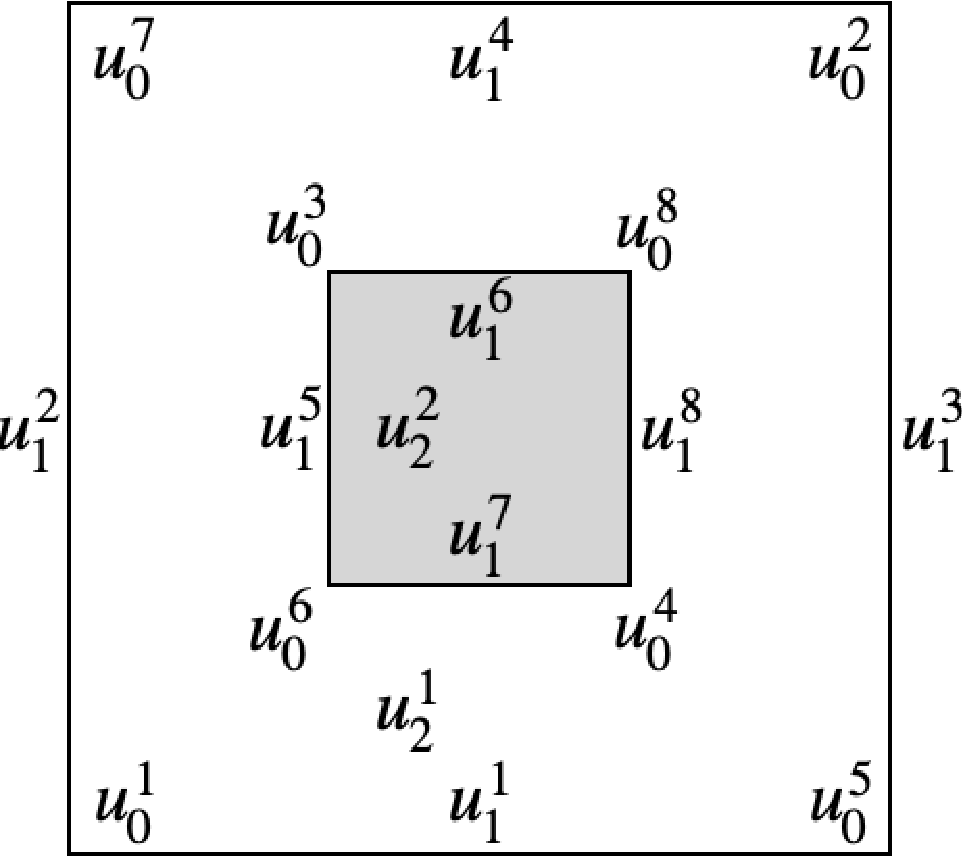
\includegraphics[width=0.4\linewidth]{~/Documents/dev/Plasm-book/chapter-03/figs/square-0.pdf} 
   \caption{Cellular 2-complex with two 2-cells, eight 1-cells, and eight 0-cells.}
   \label{fig:squares}
\end{figure}

A user-readable representation of the geometric complex $(X_2,\nu)$ is given below. |V| is the array of vertices, that provides the embedding map $C_0\to\E^2$, implemented as array $\nu: \N\to\R^2$. |EV| and |FV| respectively provide the \emph{canonical} (sorted) LAR  of 1-cells and 2-cells as lists of lists of 0-cells indices. These can be interpreted as user-readable CSR (Compressed Sparse Row) characteristic matrices $M_1$ and $M_2$ of the 0-generators of 1-cells and 2-cells, respectively, according to~\cite{Dicarlo:2014:TNL:2543138.2543294}.

\begin{lstlisting}[language=JuliaLocal, style=julia, mathescape = true]
V = [[0.,0.],[3,3],[1,2],[2,1],[3,0],[1,1],[0,3],[2,2]]
FV = [[1,2,3,4,5,6,7,8],[3,4,6,8]]
EV = [[1,5],[1,7],[2,5],[2,7],[3,6],[3,8],[4,6],[4,8]]
\end{lstlisting}

The unsigned matrix of the boundary operator $\partial_2 : C_2\to C_1$, computed by filtering elements of value 2 in the matrix $M_1 M_2^t$, is:
\[\small
[\partial_2] = \mbox{filter}(M_1M_2^t,2) = \mbox{filter}\left(\ 
\mat{
1 & 0 & 0 & 0 & 1 & 0 & 0 & 0\\
1 & 0 & 0 & 0 & 0 & 0 & 1 & 0\\
0 & 1 & 0 & 0 & 1 & 0 & 0 & 0\\
0 & 1 & 0 & 0 & 0 & 0 & 1 & 0\\
0 & 0 & 1 & 0 & 0 & 1 & 0 & 0\\
0 & 0 & 1 & 0 & 0 & 0 & 0 & 1\\
0 & 0 & 0 & 1 & 0 & 1 & 0 & 0\\
0 & 0 & 0 & 1 & 0 & 0 & 0 & 1}\,\ 
\mat{
1 & 0\\
1 & 0\\
1 & 1\\
1 & 1\\
1 & 0\\
1 & 1\\
1 & 0\\
1 & 1\\
}\,,\ 2\right)=
\mat{
1 & 0\\
1 & 0\\
1 & 0\\
1 & 0\\
1 & 1\\
1 & 1\\
1 & 1\\
1 & 1\\
}
\]
where the first column represents the non-convex 2-cell with the hole, and the second column  represents the convex cell within the hole. The reader may easily check that the four ones in positions from fifth to eighth in the second column of $[\partial_2]$ correspond to the last four unit 1-chains in \texttt{EV} array.
By multiplication $(\mbox{mod 2})$ of $[\partial_2]$ times the coordinate representation $[c]$ of the 2-complex in Figure~\ref{fig:squares}, \emph{i.e.}, times the \emph{total} 2-chain $ c = u_2^1 + u_2^2 = \vet{1 & 1}^t$, we get the coordinate representation
\[
[\partial_2][c] = \vet{1 & 1& 1& 1& 0& 0& 0& 0}^t
\]
of the 1-boundary of  $c$, \emph{i.e.}, the cycle $u_1^1 + u_1^2 + u_1^3 + u_1^4$ made by the first four 1-cells in \texttt{EV}. 
\end{coding}




\section{Cochain integration (surface, volume, inertia)}\label{sect:3-4}

The \emph{space} $C^k$ of cochains on $X$ is the dual space $(C_k)^* = \{\phi : C_k \to \R\}$ of real-valued linear integration functions on chains, i.e., on subsets of cells of the same dimension that decompose $X$.  

A \emph{domain integral} is the value that a given cochain takes on when evaluated on a given chain. This value depends bilinearly on the pair (cochain, chain). Therefore, the cochain is not the value of the integral, but the operation of calculating the integral, i.e. the application that associates (linearly) the value of the integral with each chain.

The canonical example of cochain use is the domain integration on a curve, surface, volume, solved as summation of discrete integral values (real numbers) on the 1-, 2-, or 3-dimensional cells decomposing the domain.

From the beginning of development of PLaSM as a language for solid modeling, we have introduced methods for integration of monomials on geometric shapes. In particular, they allow for surface and volume integration using a boundary triangulation, and for curve integration.  The integral on monomials may be extended easily to polynomials by linearity of both the integral and the integrand function. They can be used in |Plasm| as explained in this section. A very simple example follows.


\begin{coding}[Volume of a cube from boundary triangles.]\\
The variable |obj| first contains the memory pointer to an object of type |Hpc|, then to an object of type |Lar|. 
\begin{lstlisting}[language=JuliaLocal, style=julia, mathescape = true]
obj = SIMPLEX(3) 		#=
Hpc(MatrixNd(4), Geometry([[0.0, 0.0, 0.0], [1.0, 0.0, 0.0], [0.0, 1.0, 0.0], [0.0, 0.0, 1.0]], hulls=[[1,2,3,4]])) =#		
obj = LAR(SIMPLEX(3)) 	#=
Lar(3, 3, 4, [0.0 1.0 0.0 0.0; 1.0 0.0 0.0 0.0; 0.0 0.0 0.0 1.0], Dict{Symbol, AbstractArray}(:CV => [[1, 2, 3, 4]], :FV => [[1, 2, 3], [2, 3, 4], [1, 3, 4], [1, 2, 4]], :EV => [[2, 3], [1, 3], [1, 2], [3, 4], [2, 4], [1, 4]])) =#	
FV = obj.C[:FV]  #=
4-element Vector{Vector{Int64}}:
 [1, 2, 3]
 [1, 2, 4]
 [1, 3, 4]
 [2, 3, 4]   =#
P = (obj.V, FV); VOLUME(P)  #=
0.16666666666666666   =#
volume(P) * 6   #=
1.0   =#
\end{lstlisting}
Here, |obj.C| gives the dictionary |C| of |obj| chain bases, where |C[:FV]| denotes the array of boundary faces (triangles).
\end{coding}

%1234567890234567890234567890234567890234567890234567890234567890234567890

\subsection*{Plasm integration}\label{sect-3.4.1}


\subsubsection*{Curve integration}\label{sect-3.4.1.1}


\subsubsection*{Surface integration}\label{sect-3.4.1.2}


\subsubsection*{Volume integration}\label{sect-3.4.1.3}


